\typeout{-------------------------------- CHUNKING ----------------------------------}
\chapter{Procedural Knowledge Learning}
\label{CHUNKING}
\index{chunking}
\index{chunk}
\index{result}
\index{subgoal}

% ----------------------------------------------------------------------------
% ----------------------------------------------------------------------------
\section{Chunking}

\textit{Chunking} is Soar's experience-based mechanism for learning new procedural knowledge.  Chunking utilizes Soar's impasse-driven model of problem decomposition into sub-goals to create new productions dynamically during task execution.  These new productions, called \textbf{chunks}, summarize the substate problem-solving that occurred which led to new knowledge in a superstate.  Whenever a rule fires and creates such new superstate knowledge, which are called \textbf{results}, Soar learns a new rule and immediately adds it to production memory.  In future similar situations, the new chunk will fire and create the appropriate results in a single step, which eliminates the need to spawn another subgoal to perform similar problem-solving.  In other words, rather than contemplating and figuring out what to do, the agent immediately knows what to do.  

Chunking can effect both speed-up and transfer learning.  A chunk can effect speed-up learning because it compresses all of the problem-solving needed to produce a result into a single step.  For some real-world agents, hundreds of rule firings can be compressed into a single rule firing.  A chunk can effect transfer learning because it generalizes the problem-solving in such a way that it can apply to other situations that are similar but have not yet been experienced by the agent.

Chunks are created whenever one subgoal creates a result in a superstate; since most Soar programs are continuously sub-goaling and returning results to higher-level states, chunks are typically created continuously as Soar runs.  Note that Soar builds the chunk as soon as the result is created, rather than waiting until the impasse is resolved.

While chunking is a core capability of Soar, procedural learning is disabled by default.  See section \ref{CHUNKING-usage} for more information about enabling and using chunking.

% ----------------------------------------------------------------------------
% ----------------------------------------------------------------------------
\section{Explanation-based Chunking}

Explanation-based chunking improves on previous versions of chunking by learning rules that are qualitatively more general and expressive.  In fact, any element of a learned rule can now be variablized, and learned rules now have the full expressive power of hand-written rules. 

Figure \ref{chunk-comparison} shows an example of an explanation-based chunk and how it differs from a chunk learned from the original algorithm.  It is interesting to note that in Soar 9.4, the arithmetic agent learns 1263 rules like the one on the left-side of the figure.  In Soar 9.6, the same agent only learns 8 rules like the one on the right because they are so much more general.

\begin{figure}
	{\footnotesize
	\begin{multicols}{2}
        	\begin{verbatim}
sp {chunk-94*process-column*apply              
    (state <s1> ^operator <o1>                
                ^arithmetic-problem <a1>      
                ^one-fact 1                 
                ^top-state <s1>
                ^arithmetic <a2>
                ^arithmetic <a3>)
                
    (<o1> ^name process-column)
    (<a1> ^operation subtraction
          ^current-column <c1>)
    (<c1> -^new-digit1 <n1>
          ^digit1 0
          ^digit2 7
          ^next-column <n2>)
    (<n2> ^digit1 0 
          ^new-digit1 9
          ^next-column <n3>)
    (<n3> ^digit1 5  
          ^new-digit1 4)
    (<a2> ^subtraction-facts <s2>
          ^subtraction-facts <s3>
          ^subtraction-facts <s4>)
    (<a3> ^add10-facts <a4>)
    
    (<a4> ^digit1 0 
          ^digit-10 10)
          
          
    (<s2> ^digit1 10 ^digit2 1 
          ^result 9)
    (<s3> ^digit1 5 ^digit2 1 
          ^result 4)
    (<s4> ^digit1 10 ^digit2 7
          ^result 3)
    -->
    (<c1> ^result 3)}
        	\end{verbatim}
        	\columnbreak
        	\begin{verbatim}
sp {chunk-96*process-column*apply
    (state <s1> ^operator <o1>
                ^arithmetic-problem <a1>
                ^one-fact <o2>
                ^one-fact <o3>
                ^top-state <t1>
                ^arithmetic <a2>
                ^arithmetic <a3>)
    (<o1> ^name process-column)
    (<a1> ^operation subtraction
          ^current-column <c1>)
    (<c1> -^new-digit1 <n1>
          ^digit1 { <d2> < <d1> } 
          ^digit2 <d1>
          ^next-column <n2>)
    (<n2> ^digit1 { <d3> < <o3> } 
          ^new-digit1 <n3>
          ^next-column <n4>)
    (<n4> ^digit1 { <d4> >= <o2> } 
          ^new-digit1 <n5>)
    (<a2> ^subtraction-facts <s2>
          ^subtraction-facts <s3>
          ^subtraction-facts <s4>)
    (<a3> ^add10-facts <a4>
          ^add10-facts <a5>)
    (<a4> ^digit1 <d2> 
          ^digit-10 { <d5> >= <d1> })
    (<a5> ^digit1 <d3> 
          ^digit-10 { <d6> >= <o3> })
    (<s2> ^digit1 <d6> ^digit2 <o3> 
          ^result <n3>)
    (<s3> ^digit1 <d4> ^digit2 <o2>
          ^result <n5>)
    (<s4> ^digit1 <d5> ^digit2 <d1> 
          ^result <r1>)
    -->
    (<c1> ^result <r1>)}
        	\end{verbatim}
	\end{multicols}
	}
	\insertcaption{A Soar 9.4.0 chunk (left) vs. an explanation-based chunk (right) in the arithmetic demo agent}[A Soar 9.4.0 chunk vs. an explanation-based chunk]
	\label{chunk-comparison}
\end{figure}

To achieve this generality, chunking needs information about why rules matched in a substate and how those rules interacted.  This allows it to determine what is generalizable and what limits there are on those generalizations. Unfortunately, the information necessary to determine this information was not readily available in prior versions of Soar which only recorded a trace of all WMEs that were tested in the substate.  This trace, which we call the \textit{working memory trace} possesses limited explanatory information, which limited chunking to learning very specific rules in which only Soar identifiers were variablized and all other elements tested the exact values found in the working memory trace.  

To remedy this limitation and produce more general chunks, EBC instead analyzes two traces simultaneously:  the working memory trace and a corresponding trace of the hand-written rules that matched in the substate.  This new network of rule matches is called the explanation trace:

\vspace{18pt}
\begin{figure}[!h]
	\centering
	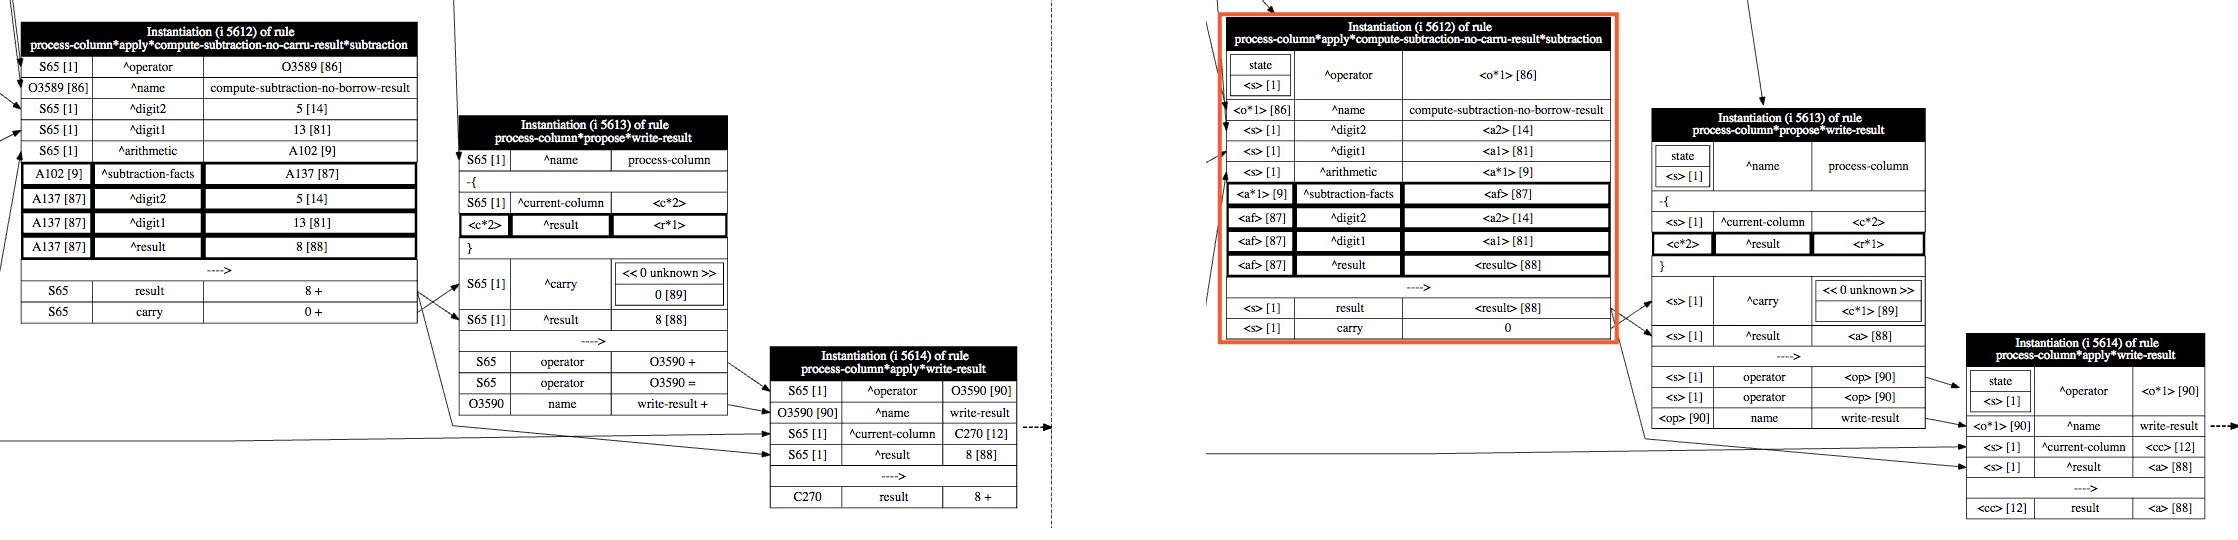
\includegraphics[width=\textwidth]{chunking-wm-vs-exp-trace.png}
	\insertcaption{A close-up of a trace showing differences between a working memory trace (left) and an explanation trace (right).  The working memory trace only contains the literal values of the WMEs that matched.  The explanation trace, on the other hand, contains variables and various constraints on the values those variables can hold.}[A comparison of a working memory trace and an explanation trace]
	\label{fig:chunking-wm-vs-exp}
\end{figure}
\vspace{6pt}

\index{instantiation}
Note that this trace is generated dynamically as rules match.  Whenever a rule matches during agent execution, Soar creates an internal record of the rule that fired, which is called a rule \textbf{instantiation}.  (Each box in the explanation traces of this chapter represents an instantiation that was created during task execution within a particular substate.) The instantiation contains both instance information about what matched (the working memory elements) and explanatory information about why they matched (the rules and actions in the original rules that contains variables, constraint tests, RHS actions, etc.).  

Note that WMEs that were automatically created by the architecture have special instantiations that explain why they were created.  For example, an architectural instantiation is created for each \soar{\carat item} attribute automatically created in operator tie impasse substates; the explanation causes the \soar{\carat item} augmentation to be dependent on the operator in the superstate that led to it, which means that chunks learned which tested that \soar{\carat item} augmentation will cause the chunk to also be dependent on the operator in the superstate.  

Similarly, architectural instantiations are created for structures recalled by semantic and episodic memory in the substate. 

\index{chunking!backtracing}
All of the instantiations that were created in a substate form the \textit{instantiation graph} of that substate.  As chunking \textbf{backtraces} through the instantiation graph, it determines the subset of instantiations that contributed to a result.  This set of instantiations and the connections between them composes the explanation trace for a learning episode.  (So, the explanation trace is a subgraph of the instantiation graph.)

\begin{figure}[!h]
	\centering
	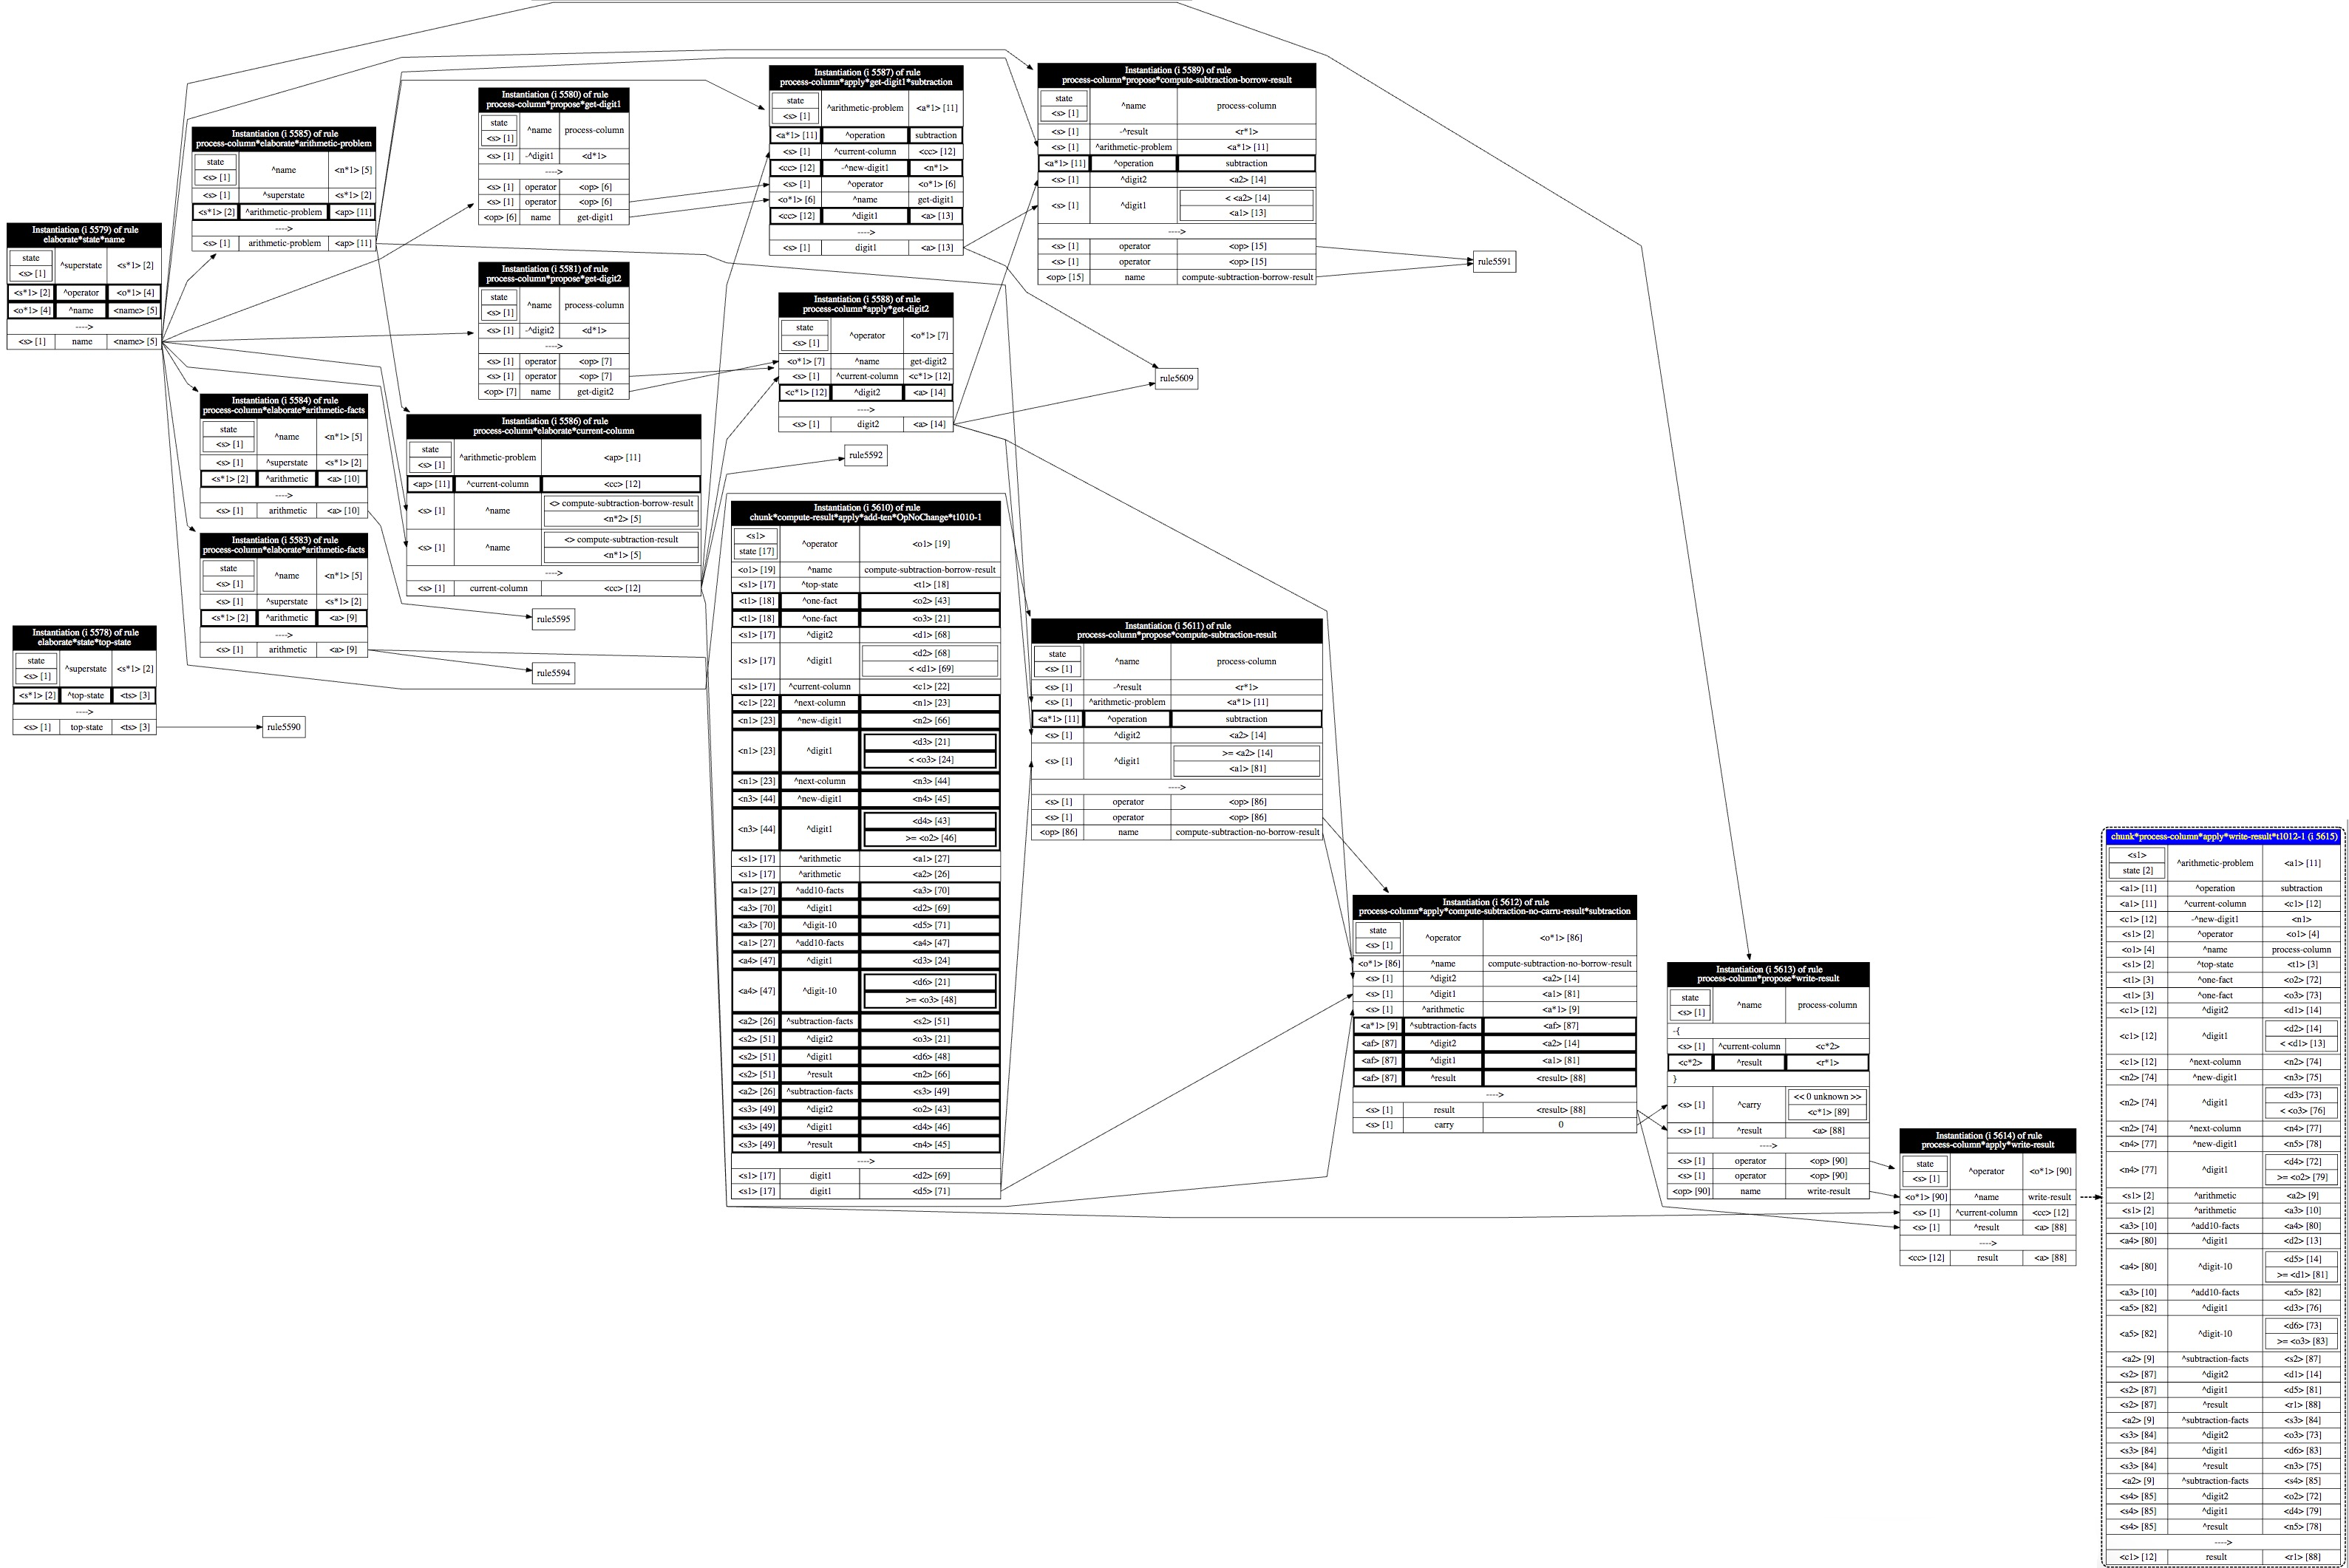
\includegraphics[width=.99\textwidth]{chunking-trace.png}
	\insertcaption{A visualization of the explanation trace of a chunk learned by the arithmetic agent.  Each box represents a rule that fired in the substate.  Arrows show dependencies between rules that create working memory elements and conditions that test those working memory elements.}[A visualization of an explanation trace]
	\label{fig:chunking-trace}
\end{figure}

EBC uses the explanation trace to determine (1) how variables were used during a problem-solving episode and (2) what constraints on those variables had to be met in order for the substate rules to match.  EBC then uses the results of this analysis to create more expressive and general rules, which can contain the full gamut of tests that hand-written rules can and can have any element variablized.


% ----------------------------------------------------------------------------
% ----------------------------------------------------------------------------
\section{Overview of the EBC Algorithm}
\label{CHUNKING-ebc}
\index{chunking!explanation-based chunking}

\textbf{Basic concepts:}

\begin{itemize}
	\item Every condition and action in the explanation trace has three \textit{elements}:
	
	\begin{itemize}
		\item For conditions, the three elements refer to the symbol in the positive equality test for the identifier, attribute and value of the condition.  For example, the last condition of rule 2 in Figure \ref{fig:chunking-trace2} has \soar{<s>} as the identifier element, number as the attribute element, and \soar{<y>} as the value element.
		
		\item For actions, the three elements refer to the identifier, attribute and value of the WME being created.
	\end{itemize}
	
	\item An element is either a variable, like  \soar{<s>}  or a literal constant, like  \soar{23},  \soar{3.3}  or  \soar{someString} .
	
\end{itemize}

% ----------------------------------------------------------------------------
\subsection{Identity}
\index{chunking!identity}

Before we can discuss the algorithm, we must first define one of its central concepts: \textit{identity}.  

\begin{itemize}
	\item \textbf{An identity is the set of all variables in a trace that refer to the same underlying object.}
	\begin{itemize}
		\item So we can say that two \textit{variables} are said to \textit{share an identity} if they both refer to the same underlying object.
	\end{itemize}
	\item \textbf{The NULL identity is a special identity that indicates an element which cannot be generalized and must contain a specific value.}
	\begin{itemize}
		\item All elements in the original rule that reference specific constant values are trivially assigned the NULL identity.
		\index{chunking!literalization}
		\item A variable's identity can also be \textit{mapped to the NULL identity}.  When this happens, we say the identity has been \textbf{literalized}.
	\end{itemize}
\end{itemize}

EBC traverses an explanation trace of the problem-solving that occurred in the substate to determine which variables in different rule instances refer to the same underlying object.  There are two ways that an explanation trace can show a shared identity:

\begin{enumerate}
	\item Variables that have the same name and are in the same rule firing will share an identity

	This is the trivial case.  The basic semantics of rules implies that the same variable in a rule references the same underlying object.

	\item If a RHS action of one rule creates a WME and a LHS condition of another rules tests that same WME, then all variables in the condition and actions will possess the same identity as their counterpart's corresponding element. 

	The interaction between the two rules indicates a shared identity between their corresponding variables.
\end{enumerate}

To get a better picture of what a shared identity is, consider the following two simple rules and the explanation trace of how they matched in a substate: 

\begin{figure}[!h]
	\centering
	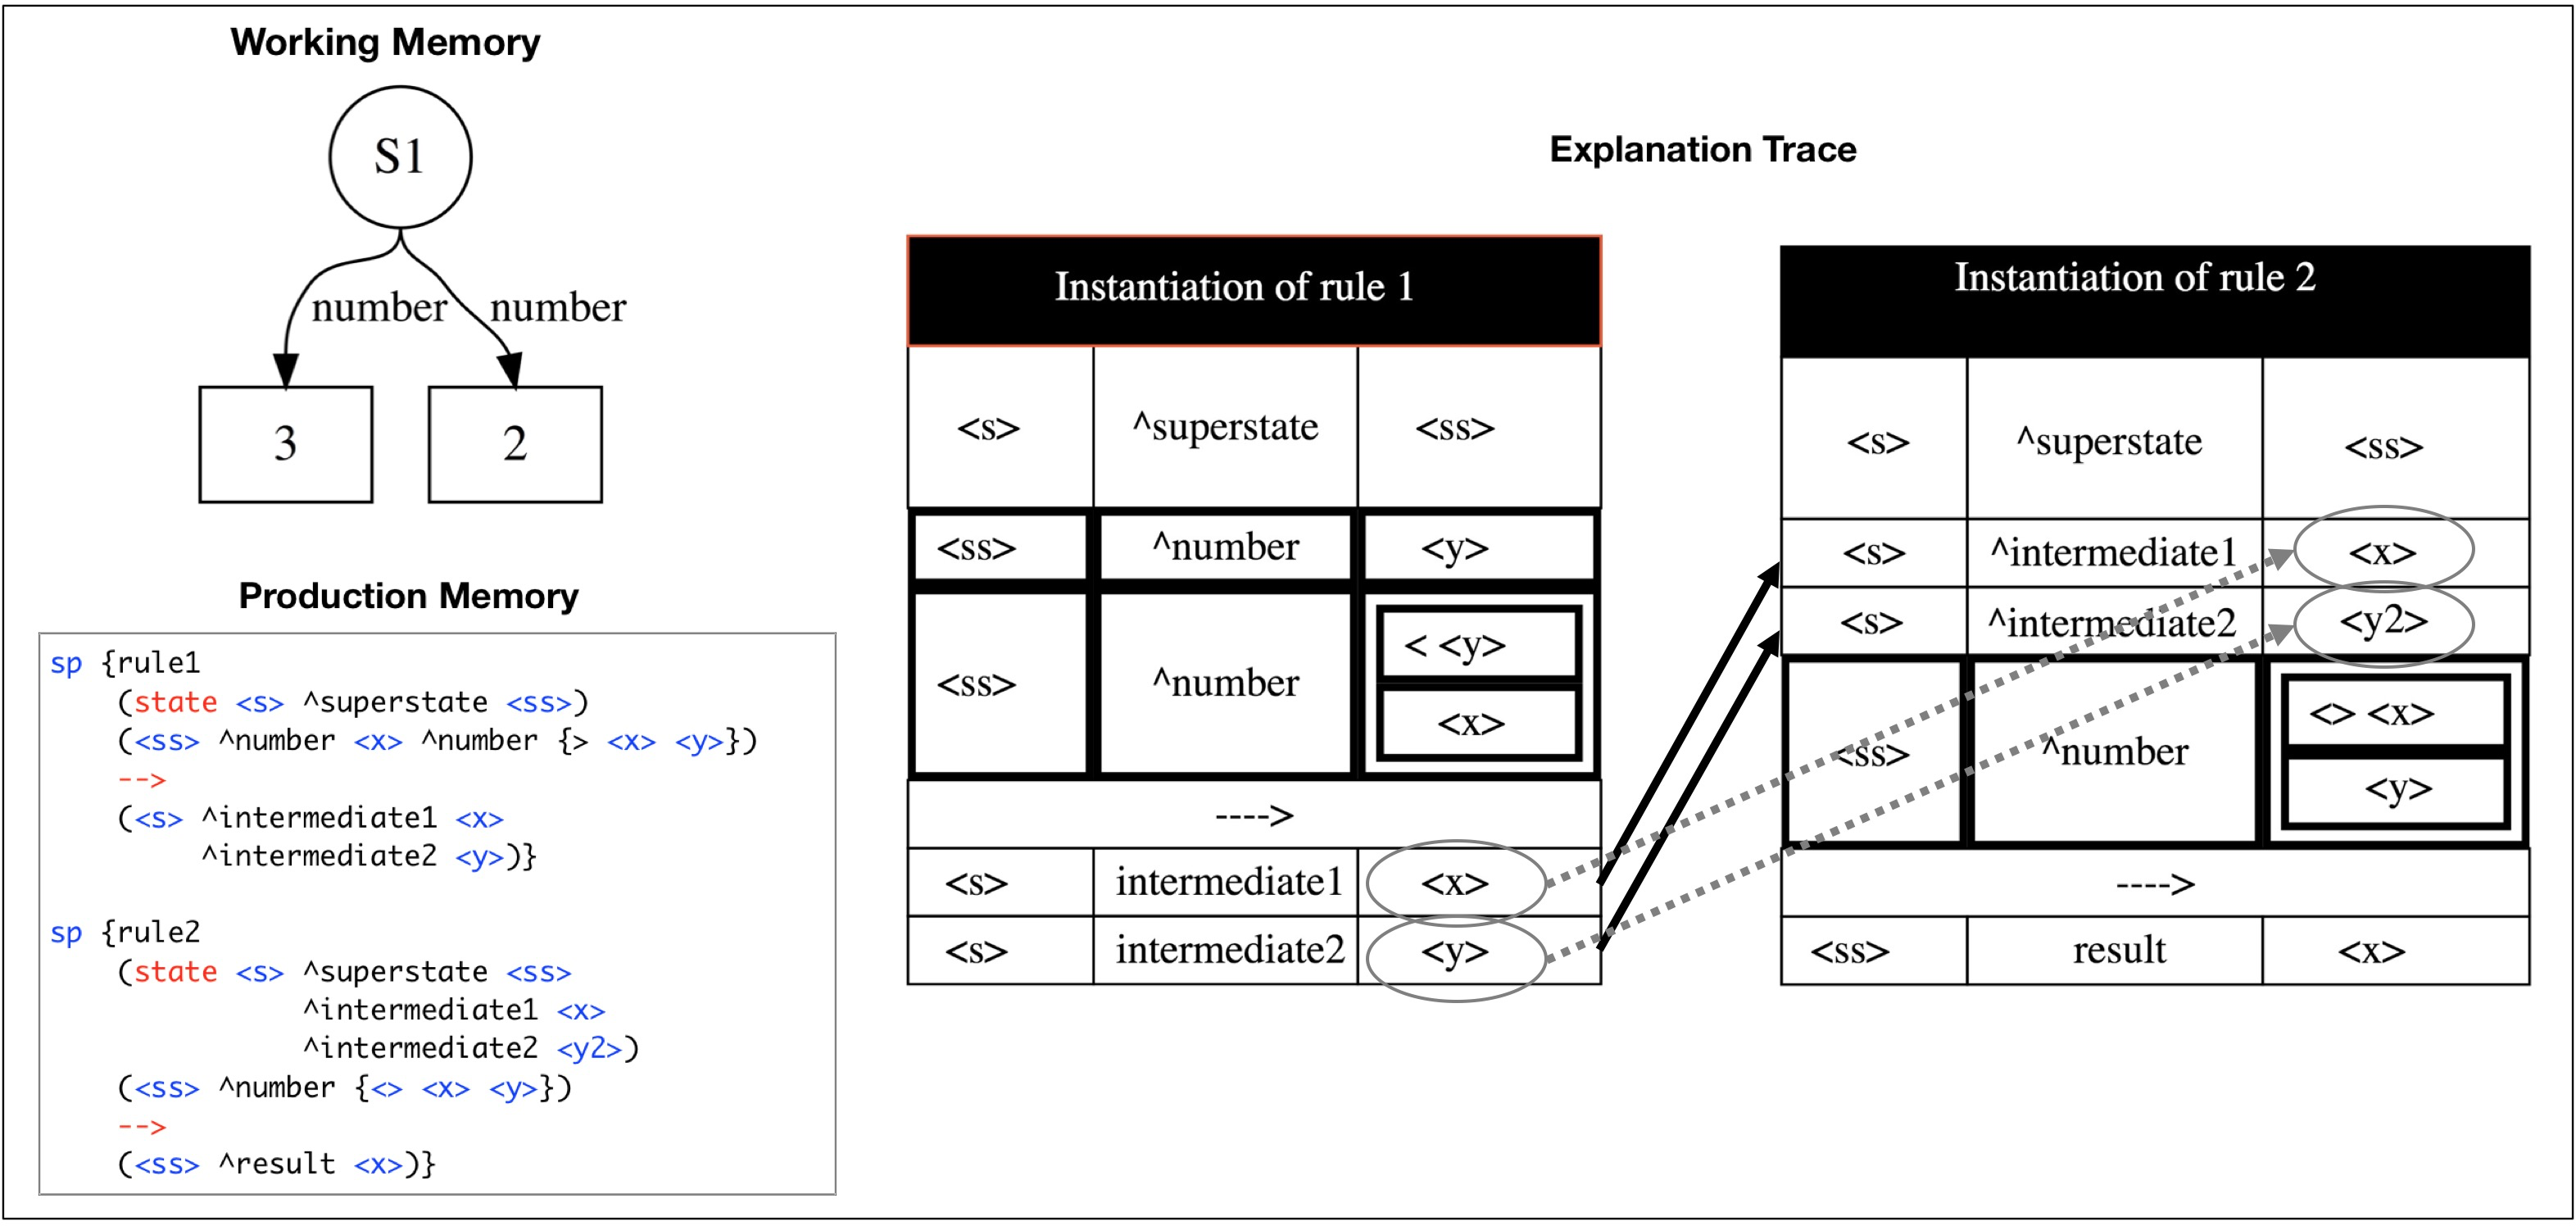
\includegraphics[width=\textwidth]{chunking-trace2.png}
	\insertcaption{An explanation trace of two simple rules that matched in a substate}
	\label{fig:chunking-trace2}
\end{figure}
\vspace{6pt}

In Figure \ref{fig:chunking-trace2}, the connection between rule 2 and rule 1 will \textit{unify} the identities of \soar{<s>}, \soar{<x>} and \soar{<y>} in rule 1 with the identities of \soar{<s>}, \soar{<x>} and \soar{<y2>} in rule 2.  So, the \soar{<x>} in rule 2 shares the same identity as the \soar{<x>} in rule 1.  Similarly, the \soar{<y2>} in rule 2 shares the same identity as \soar{<y>} in rule 1.  In contrast, the \soar{<y>} in rule 2 does NOT share the same identity as the \soar{<y>} in rule 1. 

It doesn't matter that the \soar{<y>} in rule 1 uses the same variable name as the \soar{<y>} in rule 2.  It also doesn't matter that both conditions with \soar{<y>} happen to match the same working memory element, \soar{(S1 \carat number 3)}.  In terms of sharing an identity, the only thing that matters is how the rules interact, namely whether there's a connection between elements in the condition of one rule and elements in the actions of another rule.

All literal values, for example all of the attribute in Figure \ref{fig:chunking-trace2} (\soar{superstate}, \soar{number}, \soar{intermediate1}, etc.) are considered members of the \textit{NULL identity}.

\index{chunking!literalization}
Variable identities can also be mapped to the NULL identity, which means that any elements in the final rule that share that identity will not be variablized. When this happens, we say that the identity has been \textit{literalized}.  There are two ways that a rule interaction can effect an identity literalization:

\begin{enumerate}
	\item If a RHS action of one rule creates a WME element using a constant, literal value in an element and a LHS condition tests that element, then the identity of the condition's variables is literalized and mapped to the NULL identity. 

	Because the variable in the condition matched a rule that will always create the same constant, literal value, the condition's variable must have that same value.  Otherwise, it would not have matched.
	
	
	\item If a RHS action of one rule creates a WME element using a variable and a LHS condition tests that that element is a specific value, then the identity of the action's variables is literalized and mapped to the NULL identity. 

	Because the condition requires that the rule that created the matched WME to have a specific constant, literal value, the action's variable must have that same value.  Otherwise, it would not have created something that matched the condition. 
\end{enumerate}

Identities are the basis of nearly every mechanism in explanation-based chunking.  EBC's identity analysis algorithm, which is a fairly complicated process, determines all shared identities in an explanation trace.  Figure \ref{fig:chunking-trace-identity} shows an explanation trace after identity analysis has been performed.  Elements that share an identity in the figure are colored the same.

\vspace{12pt}
\begin{figure}[!h]
	\centering
	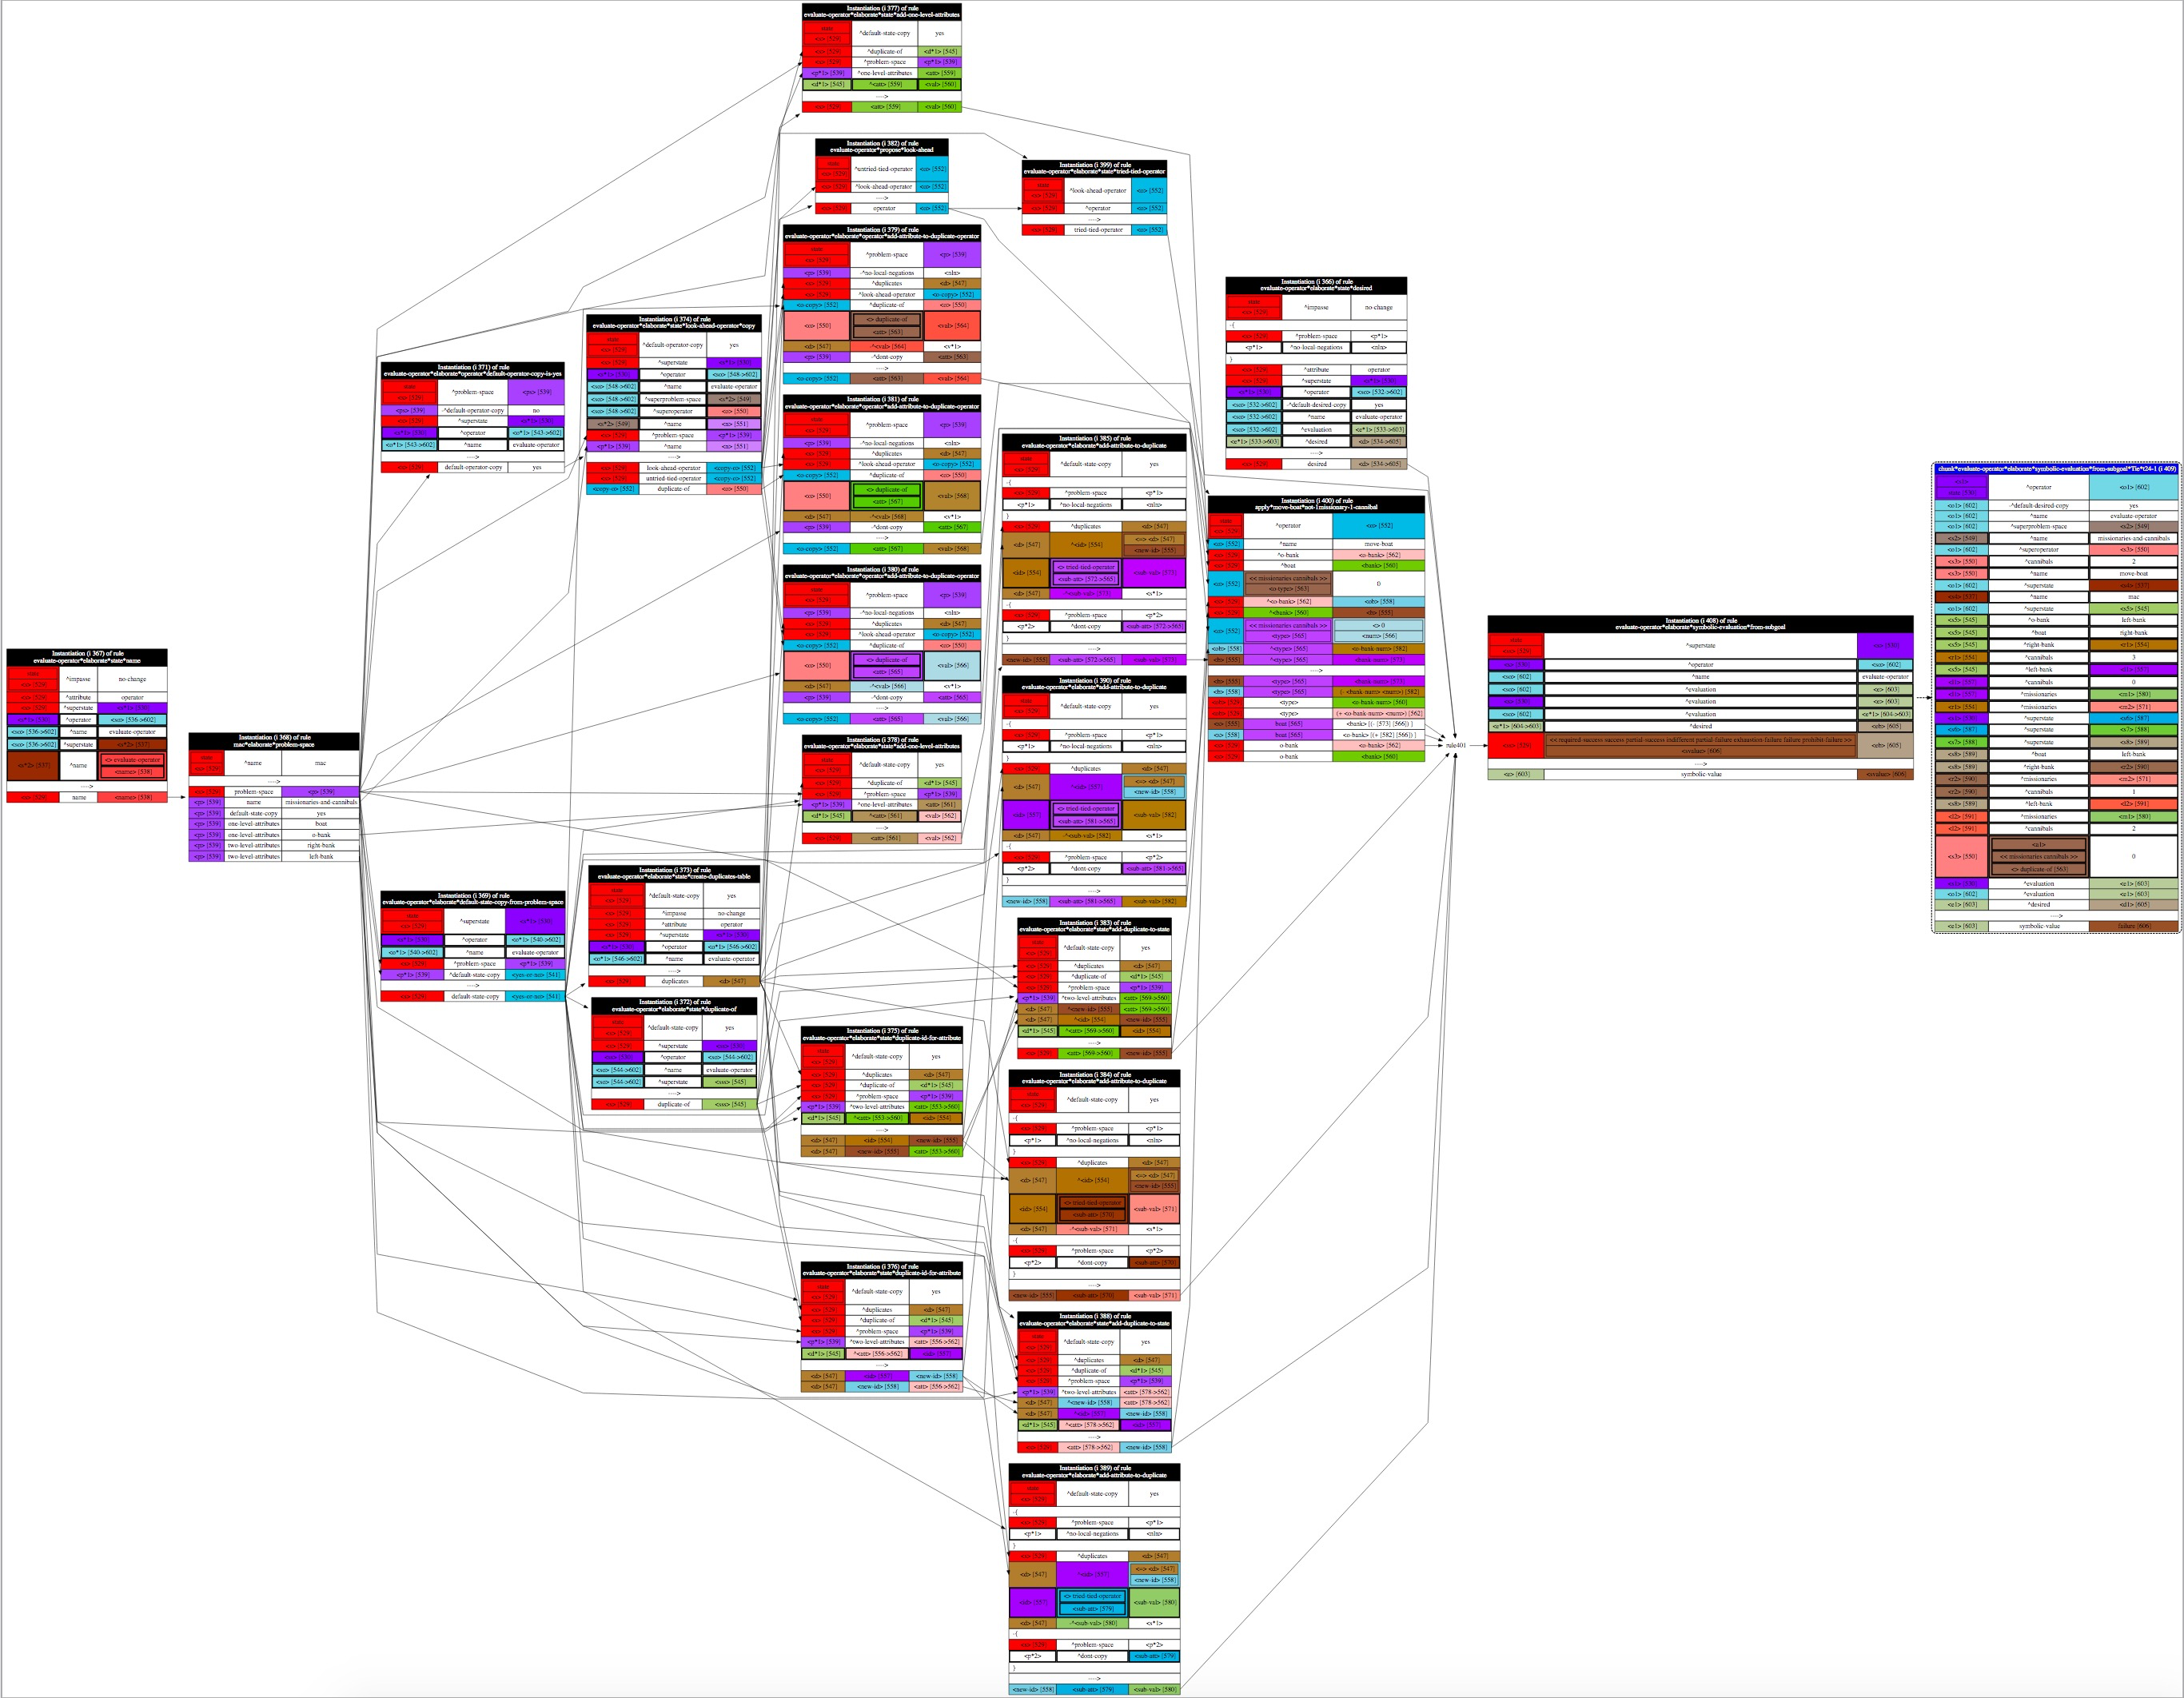
\includegraphics[width=\textwidth]{chunking-trace-identity.png}
	\insertcaption{An explanation trace after identity analysis}
	\label{fig:chunking-trace-identity}
\end{figure}

While it's not readable in this figure, note that each identity is assigned a numeric ID.  Both the explainer and the visualizer annotate elements of an explanation with the identity ID in square brackets.  These numbers are simply syntactic sugar to ease debugging and make traces easier to understand.  Underneath the hood, every test in a condition has a pointer to more complicated identity data structure that will be discussed in more detail in Section \ref{CHUNKING-prior-identities} on the identity graph. 


% ----------------------------------------------------------------------------
\subsection{The Five Main Components of Explanation-Based Chunking}
\index{chunking!ebc-components}

\vspace{12pt}
\begin{figure}
	\centering
	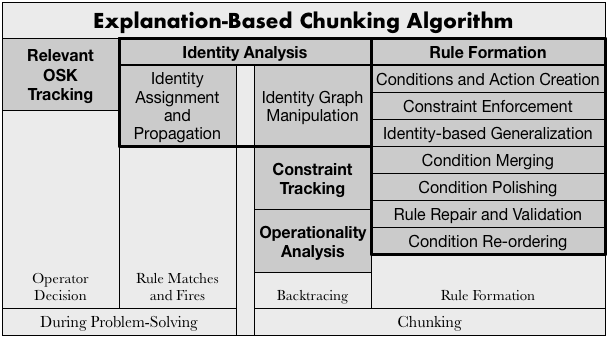
\includegraphics[width=.8\textwidth]{chunking-ebc-components.png}
	\insertcaption{Note that the two rows on the bottom indicate when each component occurs during Soar's processing.}[The five main components of explanation-based chunking]
	\label{fig:chunking-ebc-components}
\end{figure}

\begin{enumerate}
	\item \textbf{Identity analysis}  \newline
	This component determines which variables in an explanation trace share the same identity.  It also determines which identities are ineligible for variablization because they were tested against literal values in some rules.  

	Note that this component has two distinct mechanisms that occur at very different times.  The first mechanism, identity propagation, occurs constantly while problem-solving in the substate.  The second mechanism, identity graph manipulation, occurs during the learning episode.

	\item \textbf{Relevant operator selection knowledge tracking]} \newline
	This component also occurs before the learning episode.  Whenever an operator is selected, it analyzes what rule firings contributed necessary operator selection preferences and caches them in all rule instances that tests that operator. 

	\item \textbf{Constraint tracking} \newline
	This component keeps track of every value or relational constraint (e.g. \soar{<> <x>}, \soar{>= 3.14}, \soar{<< disjunction of constants >>}) placed on the various variables that share an identity.  It is used by the rule formation component to make sure that the learned rule only fires when all constraints required are met.

	\item \textbf{Operationality analysis} \newline
	This component determines which conditions in an explanation trace tested working memory elements in a superstate.  The rule formation component will use these conditions as a basis for the left-hand side of the chunk.  While it does have a few key new differences, this is the one step that is similar to previous versions of chunking.

	\item \textbf{Rule Formation} \newline
	The above four components performed the analysis that EBC needs to form a general but correct rule.  This final component uses the results of that analysis to actually build the new rule.  This is a complex component that has seven different stages.  If a valid rule is created, Soar immediately adds the rule to production memory.
\end{enumerate}

The following sections will describe each component in more detail. 


% ----------------------------------------------------------------------------
% ----------------------------------------------------------------------------
\section{What EBC Does Prior to the Learning Episode}
\label{CHUNKING-prior}
\index{result}
\index{subgoal}

While most of the work that explanation-based chunking performs occurs during the learning episode, i.e. after a rule in a substate fires and Soar detects that a result will be created, some critical aspects of the analysis it performs also occur prior to the learning episode, during problem-solving in the substate.  The two points when that happens is when a rule fires in a substate and when an operator is selected in a substate.

% ----------------------------------------------------------------------------
\subsection{Identity Assignment and Propagation}
\label{CHUNKING-prior-identities}
\index{instantiation}

Each instantiation describes the working memory elements that matched each condition and the working memory elements and preferences that are created by each action.  With the introduction of EBC, all instantiations now also store the underlying explanation behind each condition and action as defined by the original rule: which elements in conditions are variables and which ones are literal constants, which variables are the same variables, what constraints must be met on the values of each variable and any relationships between variables.

\index{chunking!identity}
EBC uses this underlying logic to determine the identities of objects used during the problem-solving.  Identities are not simply IDs.  Each identity is a declarative object that describes a set of variables across multiple rule firings and the various properties they hold. 

\emph{When an instantiation is created, EBC assigns all elements of every condition and action to an identity, creating new identities as necessary.} Identities are created and propagated using the following rules:

\begin{enumerate}
	\item If the same variable appears in multiple places in the same rule, it must be assigned the same identity.

	\item The NULL Identity is assigned to any element with a literal value in the original rule.

	\item A new identity is created and assigned for:
	\begin{enumerate}
		\item All right-hand side action elements that produce a new Soar identifier in the substate
	
		These are also known as unbound RHS variables.

		\item All variable elements of conditions that matched superstate WMEs

		It is important to note that if two conditions both match the same superstate WME, each condition is considered independent.  This means that each condition is assigned new identities for each of its elements and will produce its own condition in the final learned rule.  This is a key way that EBC differs from previous versions of chunking.
	\end{enumerate}
	\item An existing identity is propagated for:

	\begin{enumerate}
		\item Any condition element that matched a substate WME with existing identities

		Each element is assigned the identity found in the corresponding element of the action of the rule that created that WME.  This propagates identities forward through the explanation trace, which allows us to represent that the variable in the condition refers to the same object as the variable in the action of the other rule.

		\item Any element that matches special working memory elements called \textbf{singletons} are assigned the same identity.

		\label{CHUNKING-singletons1}
		\index{singleton}
		\textit{Singletons} are working memory elements that are guaranteed to only have a single possible value in a state.  The most important singleton is the local \soar{\carat superstate} singleton, which is an architecturally created WME that links the substate to the superstate, for example \soar{(S2 \carat superstate S1)}.  Since we know that it's impossible for there to be two superstate features in a state, all conditions that test that singleton WME will be assigned the same identities.

		While there are a variety of built-in singletons for architecturally-created WMEs, users can also specify their own domain-specific singletons to eliminate unnecessary generality when learning.  See section \ref{CHUNKING-usage-tuning-conditions} for more information about user singletons.  The full list of architecturally-created singletons can be found in the chunk command's help entry in section \ref{chunk}.
	\end{enumerate}
\end{enumerate}

Note that rule 1 may conflict with other rules.  For example, if a variable appears in two different conditions, then two different identities may propagate into each one of them.  In such cases, rule 1 is always enforced and propagation is ignored. During the second phase of identity analysis, which occurs during the actual learning episode, EBC will re-examine all of the condition-action pairs as it performs a backward traversal of the explanation trace and fix the missing propagations.  It does this by creating and manipulating an identity graph that can correctly incorporate all identity relationships.

% ----------------------------------------------------------------------------
\subsection{Relevant Operator Selection Knowledge Tracking}
\label{CHUNKING-prior-osk}
\index{Operator Selection Knowledge (OSK)|see{Context-Dependent Preference Set}}

As described in the beginning of this chapter, chunking summarizes the processing required to produce the results of subgoals. Traditionally, the philosophy behind how an agent should be designed was that the path of operator selections and applications from an initial state in a substate to a result would always have all necessary tests in the operator proposal conditions and any goal test, so only those items would need to be summarized. The idea was that in a properly designed agent, a substate's operator evaluation preferences lead to a more efficient search of the space but do not influence the correctness of the result. As a result, the knowledge used by rules that produce such evaluation preferences should not be included in any chunks produced from that substate.

In practice, however, it may make sense to design an agent so that search control does affect the correctness of search. Here are just two examples:

\begin{enumerate}
	\item Some of the tests for correctness of a result are included in productions that prefer operators that will produce correct results. The system will work correctly only when those productions are loaded.

	\item An operator is given a worst preference, indicating that it should be used only when all other options have been exhausted. Because of the semantics of worst, this operator will be selected after all other operators; however, if this operator then produces a result that is dependent on the operator occurring after all others, this fact will not be captured in the conditions of the chunk.
\end{enumerate}

\index{chunking!correctness}
\index{chunking!relevant operator selection knowledge}
In both of these cases, part of the test for producing a result is \emph{implicit} in search control productions. This move allows the explicit state test to be simpler because any state to which the test is applied is guaranteed to satisfy some of the requirements for success. However, chunks created in such a problem space will not be correct because important parts of the superstate that were tested by operator evaluation rules do not appear as conditions. The chunks would not accurately summarize the processing in that problem state.  The tracking of \textbf{Relevant Operator Selection Knowledge} (ROSK) is a way to address this issue.

\index{chunking!backtracing}
Relevant operator selection knowledge is the set of necessary operator evaluation preferences that led to the selection of an operator in a subgoal.  As previously described, whenever Soar learns a rule, it recursively backtraces through rule instances to determine which conditions to include in the final chunk or justification. With the ROSK, not only does Soar backtrace through each rule instance that created a matched working memory element, but it also backtraces through every rule instance that created preferences in the ROSK for any operator that gave those matched WMEs o-support. By backtracing through that additional set of preferences at each step of the backtrace, an agent will create more specific chunks that incorporate the goal-attainment knowledge encoded in the operator evaluation rules.

Specifically, this component does two things:

\begin{enumerate}
	\item When an operator is selected, it analyzes the operator preferences that led to the decision, and caches any operator selection knowledge that played a necessary role in the selection. 

	All necessity preferences, i.e. prohibit and require preferences, are always included in the ROSK since they inherently encode the correctness of whether an operator is applicable in a problem space. In contrast, some desirability preferences (rejects, betters, worses, bests, worsts and indifferents) are included in the ROSK depending on the role they play in the selection of the operator. 

	How Soar determines which of those preferences to include in the ROSK is determined by the preference semantics it uses to choose an operator. During the decision phase, operator preferences are evaluated in a sequence of seven steps or filters, in an effort to select a single operator, as described in Section \ref{PREFERENCES}.  Each step, or filter, handles a specific type of preference.  As the preference semantics are applied at each step to incrementally filter the candidate operators to a potential selected operator, EBC incrementally adds operator preferences to the ROSK based on the preferences that were instrumental in applying each filter.  A more detailed explanation of the logic used at each step can be found in Section \ref{CHUNKING-subtleties-osk}.

	\item When an o-supported rule matches, EBC caches the operator's ROSK in the instantiation of that rule.  

	Since that selection knowledge was necessary to select the operator needed for the rule to match, chunking must backtrace through that knowledge.  The operationality analysis component uses the cached ROSK to do this and incorporate the necessary operator selection reasoning knowledge into the learned rule.  For some types of agent designs, including operator selection knowledge is needed to ensure correctness.
\end{enumerate}


% ----------------------------------------------------------------------------
% ----------------------------------------------------------------------------
\section{What EBC Does During the Learning Episode}
\label{CHUNKING-during}

All of the previously discussed steps occurred during problem-solving in the substate as rules matched and operators were selected.  It is worth noting that the analysis performed prior to the learning episode is persistent and can be shared across learning episodes.  In other words, EBC can repeatedly re-use that analysis if it learns multiple chunks in the same substate.  

Every time a rule fires in a substate, Soar checks to see if any of the working memory elements created by the rule qualify as results.  This is when the actual learning episode begins.

% ----------------------------------------------------------------------------
\subsection{Calculating the Complete Set of Results}
\label{CHUNKING-during-results}
\index{result}

A chunk's actions are built from the results of a subgoal. A \textbf{result} is any working memory element created in the substate that is linked to a superstate. A working memory element is linked if its identifier is either the value of a superstate WME, or the value of an augmentation for an object that is linked to a superstate.

The results produced by a single production firing are the basis for creating the actions of a chunk. A new result can lead to other results by linking a superstate to a WME in the substate. This WME may in turn link other WMEs in the substate to the superstate, making them results. Therefore, the creation of a single WME that is linked to a superstate can lead to the creation of a large number of results. All of the newly created results become the basis of the chunk's actions.

% ----------------------------------------------------------------------------
\subsection{Backtracing and the Three Types of Analysis Performed}
\label{CHUNKING-during-backtracing}
\index{chunking!backtracing}

When learning a new rule, EBC performs a dependency analysis of the productions that fired in a substate -- a process called backtracing. Backtracing works as follows.  For each instantiated production that creates a subgoal result, backtracing examines the explanation trace to determine which working memory elements matched each condition. If the working memory element is local to the substate, then backtracing recursively examines the instantiation that created that condition's matched working memory element. Thus, backtracing traces backwards through all rules that fired and created working memory elements that were used to produce a result.

If an instantiation being backtraced through tested a selected operator, EBC will backtrace through each instantiation that created a preference in that operator's relevant operator selection knowledge set.  This behavior is off by default and can be enabled with \soar{chunk add-osk on} (See Section \ref{chunk-add-osk}.)

Multiple components of EBC perform their work during backtracing:  operationality analysis, identity analysis and constraint tracking.  The following sections will discuss what aspects of the agent's problem-solving are analyzed during backtracing.

\subsubsection{Operationality Analysis}
\label{CHUNKING-during-backtracing-operationality}

The traditional core function of chunking's backtracing is to determine which conditions in the working memory trace tested working memory elements accessible to the superstate.  These conditions will form the left-hand side of the rule.

The determination of which conditions to include is analogous to the concept of \textit{operationality} in explanation-based techniques. In classic EBL literature, operationality is typically defined as nodes in the explanation trace that are ``efficiently calculatable''.  In terms of Soar's problem-state computational model, operationality can be defined as any condition that tests knowledge linked to a superstate.  

As EBC is backtracing through rules that fired in a substate, it collects all of these operational conditions. Once the entire explanation trace is traversed, the operationality analysis will have determined exactly what superstate knowledge was tested during the process of creating a result, which it then uses as the basis for the left-hand side of the newly learned rule.  

\textbf{Note:} Soar 9.6.0's explanation-based approach has led to one key change to Soar's operationality analysis.  In previous versions of chunking, chunking would never add two conditions to a chunk that matched the same superstate working memory element.  This made sense because chunking was based on a generalization of the working memory trace.  More than one condition that tested the same WME would be redundant.  Explanation-based chunking, though, learns based on the reasoning within the original hand-written rules.  Since the reasoning behind each of the two conditions may be different even if they matched the same WME, EBC must always add both conditions.  (Note that there are some exceptions. See Section \ref{CHUNKING-usage-tuning-conditions} on superstate singletons and user singletons.)

\index{chunking!negated conditions}
Negated conditions are included in a trace in the following way: when a production fires, its negated conditions are fully instantiated with its variables' appropriate values. This instantiation is based on the working memory elements that matched the production's positive conditions. If the variable is not used in any positive conditions, such as in a conjunctive negation, a dummy variable is used that will later become a variable in a chunk.  If the identifier used to instantiate a negated condition's identifier field is linked to the super- state, then the instantiated negated condition is added to the trace as a negated condition. In all other cases, the negated condition is ignored because the system cannot determine why a working memory element was not produced in the subgoal and thus allowed the production to fire. 

\subsubsection{Identity Analysis}
\index{chunking!identity}

The first phase of identity analysis, forward identity propagation, occurred as rules fired and instantiations were recorded.  Unfortunately, forward propagation alone will not produce correct identities.  We previously gave one reason why this is the case -- conditions may have conflicting identities propagated forward -- but there are other, more complicated reasons as well that are beyond the scope of this document. What is important to know is that a second phase of identity analysis will be performed during backtracing that will refine and correct the limitations of the initial forward propagation of identity. This second phase achieves these corrections by building an identity graph, which represent the identities involved during problem-solving, and manipulating it as it backtraces through the explanation trace.

\subsubsection*{The Identity Graph}

The identity graph initially contains a node for each identity used in the explanation trace.  Each node can have multiple edges that point to children identities and a single directed \textit{join edge} that initially points back to itself.  As the agent backtraces through the explanation trace, EBC will manipulate the identity graph based on the condition-action pairs it encounters.

\begin{enumerate}
	\item \textbf{Joining identities} \newline 
	If a condition matches an action with a conflicting identity, EBC performs a join operation between the two identities. This chooses one identity as the \textit{joined identity} and points the join edges of the other identity and any previously joined identities to the new \textit{joined identity}.

	Note that any time EBC uses an element's identity, it is actually using the \textit{joined identity}.
	
	\item \textbf{Literalizing identities} \newline
	If a condition/action with a variable element matches an action/condition with a literal element, EBC marks the identity as \textit{literalized}.  This means that any conditions in the final chunk that have elements with that identity will be considered to have the NULL identity, just like constants, and will not be variablized.  Instead, the matched value will be used for that element.
	\index{chunking!NULL identity}
\end{enumerate}

\subsubsection{Constraint Tracking}
\index{chunking!correctness}
\index{chunking!over-general}

Our definition of operationality is very clear and allows us to almost trivially determine which conditions we should include in a learned rule, but it does have one shortcoming: non-operational conditions, which are ones that don't test working memory elements in the superstate, can transitively place constraints on the values of variables in operational conditions that \textit{will} appear in a chunk.  If our learning algorithm does not include these constraints, the learned rule can apply to situations where the previous substate reasoning could not have occurred, which means that the learned rule is over-general.

To handle this limitation, \textbf{\textit{EBC keeps track of all constraints found in \\ non-operational conditions that it encounters while backtracing}} in the following manner:

\begin{itemize}
	\item It stores constraints on the value a single identity, for example \soar{>= 0}, \soar{< 23}.
	\item It stores relational constraints between two identities, for example \soar{> <min>},  \soar{< <max>} or  \soar{<> <other>}.  
	\item EBC stores all of these constraints based on the underlying identities, not the variables used.  For example, if a variable \soar{<foo>} had the constraint \soar{<> <other>}, EBC would record that the variables that share the identity of \soar{<foo>} cannot have the same value as variables that share the identity of \soar{<other>}.
\end{itemize}

% ----------------------------------------------------------------------------
\subsection{Rule Formation}
\label{CHUNKING-during-formation}

\begin{wrapfigure}{R}{\thirdwidth}
	\insertfigure{chunking-rule-formation.png}{.9\thirdwidth}
	\caption[The seven stages of rule formation]{}
	\label{fig:chunking-rule-formation}
	\vspace{-40pt}
\end{wrapfigure}

There are seven distinct, sequential stages to rule formation.  The following sections will give a brief overview of each one.

\subsubsection{Condition and Action Creation}

This stage creates the basis for the left-hand and right-hand side of the rule.  
To create the initial conditions of the chunk, it copies all conditions in the explanation trace that were flagged as operational during backtracing.  These initial conditions contain literal values for each element.
To form the actions of the chunk, it creates copies of the actions that produced each of the result and all children of those results that came along for the ride.

\subsubsection{Enforcement of Constraints}

This stage adds all constraints on non-operational conditions that were collected during backtracing.  As previously described, each constraint is indexed in terms of the identity it constrains.  So, \textit{if the identity being constrained exists in one of the conditions of the learned rule}, EBC will enforce the constraint by adding a new test to that condition.

\index{chunking!literalization}
One situation in which attaching a constraint can be tricky occurs \textit{when the constrained identity has been literalized but the constraint itself refers to an identity that has not been literalized}, for example \soar{\{ > <x> 3 \}}.  While that constraint references a condition element that can only match a value of \soar{3}, the relationship between \soar{3} and the identity of \soar{<x>} must still hold (assuming \soar{<x>} appears in a different element somewhere else in the rule.)  Since these constraints still need to be enforced to ensure a correct rule, EBC will invert the constraint and attach it to a variable in another condition.  In this example, it would add a \soar{< 3} to some other condition with an element that had \soar{<x>}'s identity.

\subsubsection{Identity-Based Variablization}

To achieve any useful generality in chunks, identifiers of actual objects must be replaced by variables when the chunk is created; otherwise chunks will only ever fire when the exact same objects are matched.  At this point in the algorithm, all of the real work needed to determine the most general but correct variablization has already been performed by the identity analysis component.  

So, this step simply needs to replace all elements with non-NULL identities with variables, making sure that elements with the same joined identity are assigned the same variable.  This step also makes sure to skip and elements with identities that have been flagged as \textit{literalized}.

\subsubsection{Merging Redundant Conditions}

Any two conditions in the learned rule that share the same identities in all three elements can be combined.  In such cases, it is logically impossible for those two conditions to match two different WMEs and cause the same rules to match in the substate.  (If the two conditions were to match two different WMEs, at least one of the other rules in the explanation trace that had unified the two conditions would not have matched.)  As a result, EBC can safely merge those two conditions without losing generality.  

\subsubsection{Polishing Conditions}

EBC polishes the conditions of the learned rule by pruning unnecessary constraints on literalized elements and replacing multiple disjunction constraints with a single simplified disjunction.

\begin{enumerate}
	\item \textbf{Merging disjunctions:} 
	If an element in a condition has two disjunction tests, the constraints will be merged into a single disjunction that contains only the shared values. \soar{\{ << a b c >> << b c d >> <x>\}} becomes \soar{\{ <<b c >> <x> \}}, because it is impossible for \soar{<x>} to be either \soar{a} or \soar{b}.  This will also eliminate any duplicate disjunctions.

	\item \textbf{Throwing out unnecessary constraints:} 
	If an element in a condition has been literalized but also has a literal constraint on its value, then the constraint is unnecessary and will be thrown out.  For example,  \soar{ <s> \^{}value \{ < 33 23 \}} becomes  \soar{ <s> \^{}value 23}.
\end{enumerate}

\subsubsection{Validating Rule and Repairing Unconnected Conditions}
\label{CHUNKING-repair}
\index{chunking!repair}
At this point, the rule is essentially formed.  Chunking must now make sure that the learned rule is fully operational and can be legally added to production memory.  A fully operational rule does not have any conditions or actions that are not linked to a goal state specified in the rule. 

If an unconnected action or condition is found, EBC will attempt to repair the rule by adding new conditions that provide a link from a state that is already tested somewhere else in the rule to the unconnected condition or action.

To repair the rule, EBC performs a search through working memory to find the shortest path of working memory elements that lead from a state identifier in the rule to a WME with the identifier in the unconnected condition or action.  A new condition is then added for every WME in that found path, which is then variablized.

Note that there may be multiple paths from a state to the unconnected identifier.  EBC does a breadth-first search, so it will find one with the shortest distance.  

\subsubsection{Re-ordering Conditions}

Since the efficiency of the Rete matcher depends heavily upon the order of a production's conditions, the chunking mechanism attempts to sort the chunk's conditions into the most favorable order. At each stage, the condition-ordering algorithm tries to determine which eligible condition, if placed next, will lead to the fewest number of partial instantiations when the chunk is matched. A condition that matches an object with a multi-valued attribute will lead to multiple partial instantiations, so it is generally more efficient to place these conditions later in the ordering.  This is the same process that internally reorders the conditions in user-defined productions, as mentioned briefly in Section \ref{ARCH-pm-structure}.


% ----------------------------------------------------------------------------
% ----------------------------------------------------------------------------
\section{Subtleties of EBC}
\label{CHUNKING-subtleties}

% ----------------------------------------------------------------------------
\subsection{Relationship Between Chunks and Justifications}
\index{justification}
\index{chunk}

Chunks are closely related to another type of rule called a \textit{justification}.  Justifications are also created when a substate creates a result for a superstate, the difference being that justifications are only built when learning is off.  These justifications are needed to decide whether the working memory elements in the result should get i-support or o-support in the superstate.  To do that, Soar needs to determine whether any rules involved in the creation of the result tested the selected operator in the superstate, which is exactly the same type of analysis that chunking does.

As a result, Soar uses a limited version of the chunking algorithm to do that.  It analyzes the substate problem-solving and learns a new, temporary rule, a ``justification'', which is added to production memory.  If this temporary rule tests an operator in the superstate, it gives the result o-support. (Note that when learning is on, a justification is not needed since the chunk will provide the correct support.)

Justifications use all the components described in the following sections and are even affected by the current chunk settings.\footnote{
	Even though they don't contain variables, justifications can be over-general because they don't incorporate enough knowledge, for example, operator selection knowledge.}
 You can even print justifications out like other rules.  The only differences between chunks and justifications are:
 
 \begin{enumerate}
	\item Every condition and action in a justification contain the literal values that matched.  Justifications contain no variables.\footnote{
		Justifications can have variables in the negated conditions and negated conjunctions of conditions.  They just don't have any variables in its positive conditions.}
	\item Justifications don't contain any of the value constraints that a chunk would have.
	\item Justifications get removed from production memory as soon as their conditions no longer match. 
 \end{enumerate}

% ----------------------------------------------------------------------------
\subsection{Chunk Inhibition}
\index{chunking!inhibition}

If a newly learned chunk was immediately added to production memory, it would immediately match with the same working memory elements that participated in its creation.  This can be problematic if the production's actions create new working memory elements.  Consider the case where a substate proposes a new operator, which causes a chunk to be learned that also proposes a new operator. The chunk would immediately fire and create a preference for another new operator, which duplicates the operator preference that was the original result of the subgoal. 

To prevent this, Soar uses \textbf{inhibition}. This means that each production that is built during chunking is considered to have already fired with an instantiation based on the exact set of working memory elements used to create it. 

Note that inhibition does not prevent a newly learned chunk from immediately matching other working memory elements that are present and creating a new instantiation.

% ----------------------------------------------------------------------------
\subsection{Chunks Based on Chunks}

When a problem has been decomposed into more than one substate, a single result can produce multiple chunks.  This process is called \textit{bottom-up chunking}.  The first chunk is produced in the substate where the problem-solving that produced the result occurred.  The next chunk is based on the implicit match of the first chunk in one of the higher level problem-spaces.  If that match is lower than the state that the result is being returned to, Soar will backtrace through the chunk match and learn a second chunk (relative to the substate that the chunk matched in).  This process continues until it learns a chunk that only creates working memory elements in the same state that it matched in.

% ----------------------------------------------------------------------------
\subsection{Mixing Chunks and Justifications}
 
If an agent is using the \soar{only} or \soar{except} setting, then justifications will be built in states where learning is disabled and chunks will be built in states where learning is enabled.  In these situations, justifications also serve another purpose:  they provide an explanation of the results for future learning episodes in states that do have learning on.  EBC does this by retaining all of the extra information that chunks have but justifications do not, namely those extra tests and how things would have been variablized.  This allows EBC to learn chunks from justifications as readily as it can from hand-written rules and other chunks.

When mixing justifications and chunks, users may want to set the explainer to record the learning episodes behind justifications.  This allows one to examine the reasoning behind a justification just like you would a chunk, which may be important if that justification later participates in the formation a chunk. See Section \ref{explain} for more information about the explainer's settings.

% ----------------------------------------------------------------------------
\subsection{Generality and Correctness of Learned Rules}
\label{CHUNKING-correctness}
\index{chunking!correctness}
\index{chunking!over-general}

Chunking is intended to produce the most general rule that is also correct. 

Generality is a measure of the space of similar situations that a rule can apply to.  A more general rule can be applied to a larger space of similar situations.  A rule is considered over-general if it can apply to situations in which the original problem-solving would have never occurred.  

Correctness is a requirement that the learned rule produces the exact same results that the original problem-solving would have produced.  In other words, if we inhibited a correct chunk so that it did not fire, the agent should subgoal, execute the same substate reasoning that it previously performed when learning the chunk, and produce the same results that the learned chunk produces.

Note that an over-general rule is an incorrect rule, but not all incorrect rules are over-general.  

% ----------------------------------------------------------------------------
\subsection{Over-specialization and Over-generalization}
\label{CHUNKING-overspecialization}
\index{chunking!over-specialization}
\index{chunking!correctness}
\index{chunking!over-general}
\index{chunking!explanation-based chunking}

Explanation-based chunking was pursued to address the main limitation of traditional chunking:  \textit{over-specialized rules} that were very specific and could not be applied to many other situations. Specifically, EBC's identity-based variablization and constraint tracking/enforcement has eliminated the core source of this issue.

The nature of EBC's algorithm does add two new situations in which rules may become over-specialized.  Section \ref{CHUNKING-rhs-functions} discusses how variables used in certain RHS functions need to be literalized to maintain correctness, which can cause overspecialization. Section \ref{CHUNKING-rule-repair} discusses how testing or augmenting a previous result creates non-operational rules that require repair, a process which may sometimes over-specialize a rule.  Note that this situation can easily be avoided and, even when it does occur, may not add much unnecessary specificity to learned rules. 

While over-specialization may no longer be a common problem, it is still possible to get over-general rules.  Several of the sources of correctness issues listed in the next section can produce over-general rules in certain situations.

% ----------------------------------------------------------------------------
\subsection{Previous Results and Rule Repair}
\label{CHUNKING-rule-repair}

An agent may learn a slightly over-specialized rule when EBC repairs a rule that has unconnected conditions, which are conditions that have an identifier that is not linked to one of the states referenced in the rule.  Such rules are illegal and cannot be added to Soar's production memory. 

\textit{Rules that require repair are caused by substate problem-solving that tests or augments a previous result.}  A previous result is a working memory element that was originally created locally in the substate but then later became a result when a rule fired and connected it to the superstate.  (At which point a chunk must have been learned.). If another substate rules later matches or augments such a previous result WME \emph{using a path relative to the local substate}, then EBC will have problems.  It will know that the WME is in the superstate -- so conditions that test the WME are considered operational and augmentations on that identifier are considered results -- but it won't know where in the superstate that working memory is located is and how it should be referenced in the learned rule, because the problem solving referenced the result relative to the local substate.

As described in Section \ref{CHUNKING-repair}, EBC repairs the rule by adding new  \textit{grounding conditions} that provide a link from a state, which is tested somewhere else in the rule, to the unconnected condition or action. It does this by searching through working memory to find the shortest path from a state to the identifier behind the unconnected element.  It then variablizes those conditions appropriately.   
\index{chunking!over-specialization}

Since the conditions are based purely on what happened to be in working memory at that point and nothing in the explanation dictated that particular path found during the search, the learned rule may be over-specialized.  The chunk will only match future situations where the previous result can be found on that same path.  Fortunately, new chunks can be learned to ameliorate this.  If a similar situation is encountered in the future, but with a different path to the unconnected element, the chunk won't fire, because the added grounding conditions won't match, which should cause the agent to subgoal and learn a similar chunk with a different set of grounding conditions.

Note that if an agent designer expects that the path to the previous result found by the search will always exist, a repaired rule should match just as generally as an unrepaired rule.

But if this is not the case, an agent designer can avoid this situation by modifying the rules that test or augment the substructure of a previous result.  \emph{If those rules are modified so that they match the previous results by referencing them relative to the superstate than the the local substate, EBC will be able create a valid rule without any repair.}

To detect when this is happening, use the \soar{chunk stats} command. (See section \ref{debugging-explanation-based-chunking} It will tell you if any of an agent's learned rules that required repair.  If you instruct the explainer to record the chunk, you can also see whether a specific chunk was repaired by looking at the chunk's individual stats

% ----------------------------------------------------------------------------
\subsection{Missing Operator Selection Knowledge}

If an agent uses rules that create operator preferences to choose amongst multiple operators in the substate, it is possible that the reasoning behind those rules needs to be incorporated in any rule learned.  This topic is discussed in greater detail in Section \ref{CHUNKING-prior-osk}.  

EBC will incorporate relevant operator selection knowledge if you enable the chunk setting \soar{add-osk}, which is off by default. (See Section \ref{chunk-add-osk}.)

% ----------------------------------------------------------------------------
\subsection{Generalizing Over Operators Selected Probabilistically}

If the problem-solving in a substate involves operators that were selected probabilistically, chunking will not be able to summarize the agent's reasoning into a correct rule.  For a rule to be correct, it must always produce the same result that the substate would have produced if the learned rule was not in production memory.  Since a different operator could have been selected which could have resulted in different problem-solving, the substate could easily produce different results than any chunk learned in that substate.

Future versions of chunking will provide an option to prevent rules from forming when a probabilistically-selected operator was chosen during problem-solving.  Until then, agent engineers can disable learning in states that involve such reasoning.

% ----------------------------------------------------------------------------
\subsection{Collapsed Negative Reasoning}
\index{chunking!negated conditions}
\index{chunking!over-general}

\emph{Over-general chunks can be created when conditions in the explanation trace test for the absence of a working memory elements in the substate.} Since there is no clear way for chunking to generate a set of conditions that describe when a given working memory element would not exist in a substate, chunking can't represent that aspect of the problem-solving. 

Chunking can include negated tests if they test for \textit{the absence of working memory elements in the superstate, though}.  So, the agent engineer can avoid using negated conditions for local substate data by either (1) designing the problem-solving so that the data that is being tested in the negation is already in the superstate or (2) making the data a result by attaching it to the superstate. This increases the number of chunks learned, but a negated condition of knowledge in the superstate can be incorporated correctly into learned rules.

Note that there are agent design patterns where local negations are perfectly safe to ignore, so Soar allows local negations by default.  In some agents, they are common enough that turning the filter on prevents any rules from being learned.  

If you suspect that a rule may be over-general because of locally negated condition, you can verify whether such a condition was encountered during backtracing by using the \soar{chunk stats} command and \soar{explain stats} command.  See Sections \ref{debugging-explanation-based-chunking} and \ref{explain-stats} for more information.  

If such chunks are problematic, turning off chunking's correctness filter \\
\soar{allow-local-negations} will force Soar to reject chunks whose problem-solving involved a local negation. 

% ----------------------------------------------------------------------------
\subsection{Problem-Solving That Doesn't Test The Superstate}
\label{CHUNKING-correctness-issues-exhaustion}
\index{chunking!over-general}

Over-general chunks can be created if a result of a subgoal is dependent on the creation of an impasse within the substate. For example, processing in a subgoal may consist of exhaustively applying all the operators in the problem space. If so, then a convenient way to recognize that all operators have applied and processing is complete is to wait for a state no-change impasse to occur. When the impasse occurs, a production can test for the resulting substate and create a result for the original subgoal. This form of state test builds over-general chunks because no pre-existing structure is relevant to the result that terminates the subgoal. The result is dependent only on the existence of the substate within a substate.

In these cases, EBC will learn a chunk with no conditions, which it will reject.  But the superstate result is still created by the substate rule that matched.  If a new rule is learned that uses that result, it will be over-general since the rule does not summarize the reasoning that led to the result, namely that all operators were exhaustively applied. 

\index{quiescence}
The current solution to this problem is a bit of a hack.  Soar allows an agent to signal to the architecture that a test for a substate is being made by testing for the \soar{\carat quiescence t} augmentation of the subgoal. If this special test is found in the explanation trace, EBC will not build a chunk. The history of this test is maintained, so that if the result of the substate is then used to produce further results for a superstate, no higher chunks will be built. 

% ----------------------------------------------------------------------------
\subsection{Disjunctive Context Conflation}
\index{chunking!disjunctive context conflation}

An incorrect rule can be learned when multiple rules fire in a substate that test different structures in the superstate \emph{but create the same WME in the substate}. For example, there may be a rule that can match the superstate in several different ways, each time elaborating the local state with a WME indicating that at least one of these qualifying superstate WMEs existed. In such a situation, the rule would fire multiple times, but the result of the rule firings will be collapsed into creating a single WME in the substate. 

If this WME is then tested to create a result on the superstate, the chunk that is subsequently created can produce different behavior than the substate would have. In the original subgoal processing, multiple matches produced one substate WME, but that one substate WME only created a single result in the superstate.  The chunk on the other hand will match multiple times for each of the items that previously created the substate WME.  And then, each one of those matches will create its own distinct result in the superstate.   Since this is different behavior than the original substate, this rule would be considered incorrect. 

If it were possible, EBC should learn a \textit{disjunctive conjunctive condition}, with each disjunction being the superstate conditions tested by each substate rule that had previously created the substate WME that was repeatedly asserted.  This is why this potential source of incorrect rules is called \textit{disjunctive context conflation}.

If this type of reasoning is needed, agents can move the conflating WME to the superstate.  The rule learned would then produce only one result regardless of the number of rules that repeatedly created that WME. 

% ----------------------------------------------------------------------------
\subsection{Generalizing knowledge retrieved from \\ semantic or episodic memory}

Generalizing problem-solving based on knowledge recalled from an external memory system can be problematic for three main reasons.

\begin{enumerate}
	\item \textbf{Knowledge can change after the learning episode} \hfill
	
	Semantic knowledge can be modified by the agent.  Different semantic knowledge can effect different problem-solving, in which case a rule based on the original problem-solving would be incorrect. 

	\item \textbf{Justification for a memory recall is opaque to agent} \hfill 
	
	EBC does not have access to the reasoning behind why a piece of knowledge was recalled from a memory system.  For example, consider the case of a semantic memory that is recalled because it has the highest level of activation at a particular time.  In a future situation, the same semantic memory may not be the most active, in which case something else would be recalled and different problem-solving could occur.  Because of that possibility, the original rule is not guaranteed to produce the same result and hence has the potential to be incorrect.  (Note that this can also occur with episodic memory queries.)

	\item \textbf{Knowledge from semantic or episodic memory recalled directly into the substate is considered local} \hfill
	
	\index{chunking!over-general}
	To understand why this is a problem, remember that a chunk's conditions are based on the conditions in the explanation trace that tested knowledge linked to a superstate.  (See section \ref{CHUNKING-during-backtracing-operationality} for more information.) If semantic or episodic memory is recalled directly into the substate, then any conditions that test that recalled knowledge is considered local to the substate and will not be included as a condition in the chunk.  So, even though the substate reasoning required some piece of semantic knowledge to exist, the chunk will not require it.  And, since the learned rule \textit{is not} incorporating some of the reasoning and constraints that involved the recalled knowledge, the rule may be over-general.

	To avoid this situation, an agent can retrieve the knowledge in a higher-level state rather than the substate in which the rule is learned.
\end{enumerate}

% ----------------------------------------------------------------------------
\subsection{Learning from Instruction}
\index{chunking!learning from instruction}

	Note that some agent designs, for example an agent that learns by instruction, can take advantage of the fact that knowledge recalled from semantic or episodic memory directly into the substate is considered local.   For such agents, a rule that is directly dependent on the instructions being in working memory would be useless.  The agent would need to get the instruction every time it wanted to perform the task again, defeating the purpose of learning by instruction.  
	
	One technique that can be used to produce a more general rule which is not directly dependent on the instruction being in working memory is to first store the instructions in semantic or episodic memory.  When the agent is in a substate that it wants to learn a rule based on the instructions, it recalls the instructions from semantic or episodic memory directly into the substate.  Because that knowledge is not linked to the superstate, any rules learned in that substate will not be directly dependent on the existence of the instructions.  
	
	Since conditions that test the recalled knowledge are not incorporated into the learned rule, it is very easy to learn over-general chunks.  To avoid this, any substate rules which test recalled knowledge must also test superstate structures that correspond to the recalled knowledge.  Doing so removes the need for the instructions to exist while avoiding over-generality by ensuring that structures in the superstate corresponding to those instructions are still being tested.  Those conditions that test superstate WMEs will be generalized and included in the chunk, but the undesired portion of the reason that they matched will not be, namely the fact that the superstate knowledge corresponded to recalled instructions.

% ----------------------------------------------------------------------------
\subsection{Determining Which OSK Preferences are Relevant}
\label{CHUNKING-subtleties-osk}
\index{chunking!backtracing}

The following outline describes the logic that happens at each step. For a more detailed description of the various filters (but not the ROSK) see Section \ref{PREFERENCES} on page \pageref{PREFERENCES}. Note that depending on the set of preferences being processed, impasses may occur at some of these stages, in which case, no operator is selected and the ROSK is emptied. Moreover, if the candidate set is reduced to zero or one, the decision process will exit with a finalized ROSK. For simplicity's sake, this explanation assumes that there are no impasses and the decision process continues.

\begin{description}
	\item [Require Filter] 
	If an operator is selected based on a require preference, that preference is added to the ROSK. The logic behind this step is straightforward, the require preference directly resulted in the selection of the operator.
	\item [Prohibit/Reject Filters]
	If there exists at least one prohibit or reject preference, all prohibit and reject preferences for the eliminated candidates are added to the ROSK. The logic behind this stage is that the conditions that led to the exclusion of the prohibited and rejected candidates is what allowed the final operator to be selected from among that particular set of surviving candidates.
	\item [Better/Worse Filter]
	For every candidate that is not worse than some other candidate, add all better/worse preferences involving the candidate.
	\item [Best Filter]
	Add any best preferences for remaining candidates to the ROSK.
	\item [Worst Filter]
	If any remaining candidate has a worst preference which leads to that candidate being removed from consideration, that worst preference is added to the ROSK. Again, the logic is that the conditions that led to that candidate not being selected allowed the final operator to be chosen.
	\item [Indifferent Filter]
	This is the final stage, so the operator is now selected based on the agent's exploration policy. How indifferent preferences are added to the ROSK depends on whether any numeric indifferent preferences exist.
	\begin{enumerate}
		\item If there exists at least one numeric indifferent preference, then every numeric preference for the winning candidate is added to the ROSK. There can be multiple such preferences. Moreover, all binary indifferent preferences be- tween that winning candidate and candidates without a numeric preference are added.
		\item If all indifferent preferences are non-numeric, then any unary indifferent preferences for the winning candidate are added to the ROSK. Moreover, all binary indifferent preferences between that winning candidate and other candidates are added.
	\end{enumerate}
	The logic behind adding binary indifferent preferences between the selected operator and the other final candidates is that those binary indifferent preferences prevented a tie impasse and allowed the final candidate to be chosen by the exploration policy from among those mutually indifferent preferences.
\end{description}

Note that there may be cases where two or more rules create the same type of preference for a particular candidate. In those cases, only the first preference encountered is added to the ROSK. Adding all of them can produce over-specific chunks. It may still be possible to learn similar chunks with those other preferences if the agent subgoals again in a similar context.

Note also that operator selection knowledge is not tracked and incorporated into chunks by default. The setting must be turned on via the chunk command's \soar{add-osk} setting. See Section \ref{chunk} on page \pageref{chunk} for more information. 

The ROSK also affects the conditions of justifications, so the \soar{add-desirability-prefs} setting does have an effect on the agent even if learning is turned off.

% ----------------------------------------------------------------------------
\subsection{Generalizing Knowledge From Math \\ and Other Right-Hand Side Functions}
\label{CHUNKING-rhs-functions}
\index{chunking!literalization}

Explanation-based chunking introduces the ability to learn more expressive rules whose actions perform arbitrary right-hand side functions with variablized arguments.  

It is important to note that this ability is limited.  EBC can only learn rules with generalized RHS functions in its actions when the rule that created the result contained a RHS function.  In many cases, RHS functions will be used in the intermediate rule firings in the explanation trace.  Not only will these intermediate RHS function not appear in the chunk, but any chunk learned based on their output will become more specific.  This is one of the sources of over-specialization referenced in section \ref{CHUNKING-overspecialization}.
 
RHS function calls in intermediate rule firings are a challenge for EBC to deal with because the problem-solving may have placed constraints on the intermediate results that cannot be represented in a single Soar rule.  

For example, consider the case of one rule that used a RHS function to add two numbers.  Now consider another rule that matched the output of the RHS function, but only if it was less than 5.  If the second rule matched, it would return the total as a result.  How could we encode the reasoning of those two rules into one rule?  Since Soar's production syntax does not allow using RHS function as constraints in conditions, there is no way to insure that the two numbers add up to something less than 5 in a single rule.  This is why RHS functions in intermediate rule firings can cause over-specialization.  

Because the chunk's conditions can't represent constraints on the output of intermediate RHS functions, EBC must literalize both the identities of the variables that appear as arguments to the intermediate RHS function, as well as the identities in any conditions that test the output of the RHS function.  That fixes the value of the RHS function and guarantees that any constraints in conditions that test the output of that RHS function will be met.  While this will make the learned rule more specific, it will also ensure that the rule is correct.

% ----------------------------------------------------------------------------
\subsection{Situations in which a Chunk is Not Learned}

Soar learns a chunk every time a subgoal produces a result, unless one of the following conditions is true:

\begin{enumerate}
	\item \textbf{Chunking is off} 
	
	This corresponds to the command \soar{chunk never}.  See Section \ref{chunk} on page \pageref{chunk} for details of \soar{chunk} and how to turn chunking on or off.

	\index{chunking!RHS functions}
	\index{RHS Function!dont-learn}
	\index{RHS Function!force-learn}
	\item \textbf{Chunking was only enabled for some states, and the subgoal in question is not one of them}
	
	When chunking is enabled via the \soar{only} or \soar{except} command, the agent must specify which states learning either occurs in or doesn't occur in, respectively.  For the \soar{except} setting, Soar will learn rules in all states in which a \soar{dont-learn} RHS production action was not executed.  Similarly, for the \soar{only} setting, Soar will learn rules in all states where a \soar{force-learn} RHS production action was executed.  See Section \ref{SYNTAX-pm-rhs-learning} on page \pageref{SYNTAX-pm-rhs-learning} for more information.

	This capability is provided for debugging and practical system development, but it is not part of the theory of Soar.

	\item \textbf{The chunk learned is a duplicate of another production or chunk already in production memory}

	In some rare cases, a duplicate production will not be detected because the order of the conditions or actions is not the same as an existing production.

	\index{chunking!correctness}
	\item \textbf{The problem-solving in the substate violated one of the enabled correctness guarantee filters}

	During the development of explanation-based chunking, we have developed a list of possible causes of incorrect chunks. EBC's correctness guarantee filters detect when those situations occur and prevents a chunk from being learned.  

	\index{chunking!over-general}
	For example, the \soar{allow-local-negations} filter will prevent a rule from being formed if the problem-solving that led to the result was dependent on a condition that tested whether a subgoal WME doesn't exist.  Since there is no practical way to determine why a piece of knowledge doesn't exist, testing a local negation can result in an over-general and incorrect chunk.  See Section \ref{CHUNKING-usage-tuning-correctness} on page \pageref{CHUNKING-usage-tuning-correctness} for more information. 

	Note that correctness filters have not yet been implemented for all the identified potential sources of correctness issues.

	\item \textbf{The chunking option \soar{bottom-only} is on and a chunk was already built in the bottom subgoal that generated the results}

	With \soar{bottom-only} chunking, chunks are learned only in states in which no subgoal has yet generated a chunk. In this mode, chunks are learned only for the ``bottom'' of the subgoal hierarchy and not the intermediate levels. With experience, the subgoals at the bottom will be replaced by the chunks, allowing higher level subgoals to be chunked .  See Section \ref{chunk} on page \pageref{chunk} for details of chunk used with the \soar{bottom-only} setting.

	\index{quiescence}
	\item \textbf{The problem-solving that led to the result contained a condition that tested the architecturally-created \soar{<state> \carat quiescence t} augmentation}

	This mechanism is motivated by the \textit{chunking from exhaustion} problem, where the results of a subgoal are dependent on the exhaustion of alternatives (see Section \ref{CHUNKING-correctness-issues-exhaustion} on page \pageref{CHUNKING-correctness-issues-exhaustion}). If this substate augmentation is encountered when determining the conditions of a chunk, then no chunk will be built for the currently considered action. This is recursive, so that if an un-chunked result is relevant to a second result, no chunk will be built for the second result. This does not prevent the creation of a chunk that would include \soar{\carat quiescence t} as a condition.

	\item \textbf{The problem-solving in the substate did not test any knowledge in the superstate}

	In these cases, the chunk learned does not have any conditions and is not a legal production.  \emph{Note that this creates an unusual persistence issue for any results that came out of the substate.}  Since a justification or chunk was not learned, there is no rule in the superstate that can provide either i-support or o-support for the result that came out of the substate.   Consequently, those result WMEs will be completely dependent on the rules that fired within the substate.  So, when the substate is removed, those results will also be removed.
\end{enumerate}


% ----------------------------------------------------------------------------
% ----------------------------------------------------------------------------
\section{Usage}
\label{CHUNKING-usage}
\index{chunking!usage}

% ----------------------------------------------------------------------------
\subsection{Overview of the \soar{chunk} command}
\index{chunk (command)}

{\scriptsize
\begin{verbatim}
===================================================
           Chunk Commands and Settings
===================================================
? | help                                              Print this help listing
timers                                 [ on | OFF ]   Timing statistics (no args to print stats)
stats                                                 Print stats on learning that has occurred
------------------- Settings ----------------------
ALWAYS | never | only | except                        When Soar will learn new rules
bottom-only                            [ on | OFF ]   Learn only from bottom substate
naming-style                     [ numbered | RULE]   Simple names or rule-based name
max-chunks                                 50         Max chunks that can be learned (per phase)
max-dupes                                   3         Max duplicate chunks (per rule, per phase)
------------------- Debugging ---------------------
interrupt                              [ on | OFF ]   Stop Soar after learning from any rule
explain-interrupt                      [ on | OFF ]   Stop Soar after learning explained rule
warning-interrupt                      [ on | OFF ]   Stop Soar after detecting learning issue
------------------- Fine Tune ---------------------
singleton                                             Print all WME singletons
singleton                <type> <attribute> <type>    Add a WME singleton pattern
singleton -r             <type> <attribute> <type>    Remove a WME singleton pattern
----------------- EBC Mechanisms ------------------
add-ltm-links                          [ on | OFF ]   Recreate LTM links in original results
add-osk                                [ on | OFF ]   Incorporate operator selection knowledge
merge                                  [ ON | off ]   Merge redundant conditions
lhs-repair                             [ ON | off ]   Add grounding conds for unconnected LHS
rhs-repair                             [ ON | off ]   Add grounding conds for unconnected RHS
user-singletons                        [ ON | off ]   Use domain-specific singletons
---------- Correctness Guarantee Filters ----------   Allow rules to form that...
allow-local-negations                  [ ON | off ]   ...used local negative reasoning
allow-opaque*                          [ ON | off ]   ...used knowledge from a LTM recall
allow-missing-osk*                     [ ON | off ]   ...tested operators selected using OSK
allow-uncertain-operators*             [ ON | off ]   ...tested probabilistic operators
\end{verbatim}
* disabled
}

See Section \ref{chunk} for more detailed information about the \soar{chunk} command's settings.

% ----------------------------------------------------------------------------
\subsection{Enabling Procedural Learning}
\label{CHUNKING-usage-enable}

By default, explanation-based chunking is off.

\begin{itemize}
	\item To turn on chunking: \soar{chunk always}
	\item To turn off chunking: \soar{chunk never}
\end{itemize}

In real world agents, there may be certain problem spaces in which you don't want your agent to learn rules.  Chunking has a mechanism to allow agents to dynamically specify the states in which rules are learned. 

\begin{itemize}
	\item To turn off chunking in all states except ones manually flagged on: 
	\begin{itemize}
		\item Use \soar{chunk only} setting.
		\item Design an agent rule that executes the RHS action \soar{force-learn}, which only matches in states in which you want to learn rules.
	\end{itemize}
	\item To turn on chunking in all states except ones manually flagged off: 
	\begin{itemize}
		\item Use \soar{chunk except} setting.
		\item Design an agent rule that executes the RHS action \soar{dont-learn}, which only matches in states in which you don't want to learn rules.
	\end{itemize}
\end{itemize}

Depending on your agent design, you may want to consider enabling the \soar{add-osk} option.  As of Soar 9.6.0, EBC does not incorporate operator selection knowledge into learned rules by default, since there is a performance cost and not all agents designs require its inclusion.  You may want to enable this option if your agent has rules that test knowledge in the superstate to create operator preferences in the substate.  See section \ref{CHUNKING-prior-osk} on page \pageref{CHUNKING-prior-osk} for more information about learning and operator selection knowledge. 

See Section \ref{chunk} on page \pageref{chunk} for more information about using the chunk command to enable and disable procedural learning.


% ----------------------------------------------------------------------------
\subsection{Fine-tuning What Your Agent Learns}
\label{CHUNKING-usage-tuning}

\subsubsection{Prohibiting known sources of correctness issues}
\label{CHUNKING-usage-tuning-correctness}
\index{chunking!correctness}

It is theoretically possible to detect nearly all of the sources of correctness issues and prevent rules from forming when those situations are detected.  In Soar 9.6.0, though, only one filter is available, \soar{allow-local-negations}.  Future versions of Soar will include more correctness filters.

Note that it is still possible to detect that your agent may have encountered a known source of a correctness issue by looking at the output of the \soar{chunk stats} command.  It has specific statistics for some of the sources, while others can be gleaned indirectly.  For example, if the stats show that some rules required repair, you know that your agent testing or augmenting a previous result in a substate.

\subsubsection{Using singletons to simplify a rule's conditions}
\label{CHUNKING-usage-tuning-conditions}
\index{singleton}
\index{chunking!singleton}

Unlike previous versions of chunking, EBC adds all conditions that tested superstate knowledge to a chunk, regardless of whether another condition already tested that working memory element.  This means that EBC can sometimes produce learned rules with seemingly duplicate conditions.  While these conditions are logically correct, they may be redundant because the nature of the domain may make it impossible for the two conditions to match different working memory elements.  For example, in the blocks-world domain, the fact that there can be only one gripper in the world means that having multiple conditions testing for a gripper would be redundant.  

Soar allows agents to specify such known domain characteristics, which EBC will then use to create better rules that don't have such unnecessary conditions.  We call any working memory element that is guaranteed to only have a single possible value at any given time, a \textit{singleton}.  If EBC encounters two different conditions in the backtrace that both test the same superstate WME that matches a user singleton pattern, it will merge the two conditions. As described in Section \ref{CHUNKING-singletons1}, there are several architectural singleton's that EBC already knows about.  To specify patterns for domain-specific singletons, the \soar{chunk singleton} command can be used. 

See Section \ref{chunk} for more information about the chunk singleton command.

% ----------------------------------------------------------------------------
\subsection{Examining What Was Learned}

\subsubsection{Printing and Traces}
\index{chunking!backtracing}

\textbf{Printing Rules:}
\begin{itemize}
	\item To print all chunks learned: \newline  \soar{print --chunks} or \soar{print -c}
	\item To print all justifications learned (and still matching):  \newline \soar{print --justifications} or \soar{print -j}
	\item To print a rule or justification: \newline  \soar{print <rule-name>}
\end{itemize}

For more information on print, see section \ref{print} on page \pageref{print}.

\textbf{Trace Messages:}
\begin{itemize}
	\item To print when new rules are learned (just the name): \newline \soar{trace --learning 1} or  \soar{trace -l 1} 
	\item To print when new rules are learned (the full rule): \newline \soar{trace --learning 2} or  \soar{trace -l 2} 
	\item To print a trace of the conditions as they are collected during backtracing: \newline \soar{trace --backtracing} or  \soar{trace -b} 
	\item To print warnings about chunking issues detected while learning:  \newline \soar{trace --chunk-warnings} or \soar{trace -C}
	\item To print when learned chunks match and fire: \newline  \soar{trace --backtracing} or  \soar{trace -b} 
\end{itemize}
For more information on trace, see section \ref{trace} on page \pageref{trace}.

Note that the most detailed information about why a particular rule was learned can be acquired using the explain mechanism as described in section \ref{explain} on page \pageref{explain}.  That is highly recommended over printing the backtracing trace messages.

\subsubsection{Chunking Statistics}

Chunking automatically compiles various statistics about the procedural rule learning that an agent performs.  To access these stats, use the command \soar{chunk stats} or \soar{stats -l}

\begin{center}
{\small
\begin{verbatim}
===========================================================================
                  Explanation-Based Chunking Statistics
===========================================================================
Substates analyzed                                                     0
Rules learned                                                          0
Justifications learned                                                 0

---------------------------------------------------------------------------
                               Work Performed
---------------------------------------------------------------------------
Number of rules fired                                                  0
Number of rule firings analyzed during backtracing                     0
Number of OSK rule firings analyzed during backtracing                 0
Number of rule firings re-visited during backtracing                   0

Conditions merged                                                      0
Disjunction tests merged                                               0
- Redundant values                                                     0
- Impossible values eliminated                                         0

Operational constraints                                                0
Non-operational constraints detected                                   0
Non-operational constraints enforced                                   0

---------------------------------------------------------------------------
                           Identity Analysis
---------------------------------------------------------------------------
Identities created                                                     0
Distinct identities in learned rules                                   0
Identity propagations                                                  0
Identity propagations blocked                                          0
Identity propagations from local singleton                             0
Identities joined                                                      0
- To unify two identities propagated into same variable                0
- To unify two conditions that tested a superstate singleton           0
- To connect an child result (result in rule had children WMEs)        0
Identities literalized                                                 0
- Condition with variable matched a literal RHS element                0
- Condition with variable matched a RHS function                       0
- Condition with literal value matched a RHS variable                  0
- Variable used in a RHS function                                      0

---------------------------------------------------------------------------
                  Potential Generality Issues Detected
---------------------------------------------------------------------------
Rules repaired that had unconnected conditions or actions              0
Extra conditions added during repair                                   0

---------------------------------------------------------------------------
                  Potential Correctness Issues Detected
---------------------------------------------------------------------------
Chunk used negated reasoning about substate                            0
Chunk tested knowledge retrieved from long-term memory                 0
Justification used negated reasoning about substate                    0
Justification tested knowledge retrieved from long-term memory         0

---------------------------------------------------------------------------
                      Learning Skipped or Unsuccessful
---------------------------------------------------------------------------
Ignored duplicate of existing rule                                     0
Skipped because problem-solving tested ^quiescence true                0
Skipped because no superstate knowledge tested                         0
Skipped because MAX-CHUNKS exceeded in a decision cycle                0
Skipped because MAX-DUPES exceeded for rule this decision cycle        0
\end{verbatim}
}
\end{center}

Note that similar statistics for a specific learned rule can be acquired using the explain mechanism as described in section \ref{explain} on page \pageref{explain}.

\subsubsection{Interrupting Execution To Examine Learning}

\begin{itemize}
	\item To stop Soar after each successful learning episode: \newline \soar{chunk interrupt on} 
	\item To stop Soar after detecting any learning issue: \newline \soar{chunk warning-interrupt on} 
	\item To stop Soar after learning a rule that the explainer recorded: \newline \soar{chunk explain-interrupt on} 

For more information about how to record when a specific rule is leared, see section \ref{explain} on page \pageref{explain} that describes the explain mechanism.

\end{itemize}


% ----------------------------------------------------------------------------
% ----------------------------------------------------------------------------
\section{Explaining Learned Procedural Knowledge}

While explanation-based chunking makes it easier for people to now incorporate learning into their agents, the complexity of the analysis it performs makes it far more difficult to understand how the learned rules were formed. The explainer is a new module that has been developed to help ameliorate this problem. The explainer allows you to interactively explore how rules were learned.
 
When requested, the explainer will make a very detailed record of everything that happened during a learning episode. Once a user specifies a recorded chunk to "discuss", they can browse all of the rule firings that contributed to the learned rule, one at a time. The explainer will present each of these rules with detailed information about the identity of the variables, whether it tested knowledge relevant to the the superstate, and how it is connected to other rule firings in the substate. Rule firings are assigned IDs so that user can quickly choose a new rule to examine.

The explainer can also present several different screens that show more verbose analyses of how the chunk was created. Specifically, the user can ask for a description of (1) the chunk's initial formation, (2) the identities of variables and how they map to identity sets, (3) the constraints that the problem-solving placed on values that a particular identity can have, and (4) specific statistics about that chunk, such as whether correctness issues were detected or whether it required repair to make it fully operational.

Finally, the explainer will also create the data necessary to visualize all of the processing described in an image using the new 'visualize' command. These visualization are the easiest way to quickly understand how a rule was formed.
 
Note that, despite recording so much information, a lot of effort has been put into minimizing the cost of the explainer. When debugging, we often let it record all chunks and justifications formed because it is efficient enough to do so.

\rule{\textwidth}{1pt}

Use the \soar{explain} command without any arguments to display a summary of which rule firings the explainer is watching. It also shows which chunk or justification the user has specified is the current focus of its output, i.e.~the chunk being discussed.

Tip: This is a good way to get a chunk id so that you don't have to type or paste in a chunk name.

{\footnotesize
\begin{verbatim}
=======================================================
                   Explainer Summary
=======================================================
Watch all chunk formations                            Yes
Explain justifications                                Nof
Number of specific rules watched                      0

Chunks available for discussion:                      chunkx2*apply2 (c 14)
                                                      chunk*apply*o (c 13)
                                                      chunkx2*apply2 (c 12)
                                                      chunk*apply*d (c 11)
                                                      chunkx2*apply2 (c 6)
                                                      chunk*apply* (c 15)
                                                      chunkx2*apply (c 8)
                                                      chunk*apply*c (c 5)
                                                      chunkx2*apply (c 10)
                                                      chunk*apply (c 1)

* Note:  Printed the first 10 chunks. 'explain list' to see other 6 chunks.

Current chunk being discussed:                        chunk*apply*down-gripper(c 3)

\end{verbatim}
}

\rule{\textwidth}{1pt}

\textbf{\soar{explain chunk [ <chunk id> | <chunk name> ]}}

This command starts the explanation process by specifying which chunk's eplanation trace you want to explore.

Tip: Use the alias \soar{c} to quickly start discussing a chunk, for example:

{\tiny
\begin{verbatim}
soar % c 3
Now explaining chunk*apply*move-gripper-above*pass*top-state*OpNoChange*t6-1.
- Note that future explain commands are now relative
  to the problem-solving that led to that chunk.

Explanation Trace                                     Using variable identity IDs                  Shortest Path to Result Instantiation

sp {chunk*apply*move-gripper-above*pass*top-state*OpNoChange*t6-1
1:    (<s1> ^top-state <s2>)                          ([140] ^top-state [162])
     -{
2:    (<s1> ^operator <o*1>)                          ([140] ^operator [141])
3:    (<o*1> ^name evaluate-operator)                 ([141] ^name evaluate-operator)
     }
4:    (<s2> ^gripper <g1>)                            ([162] ^gripper [156])                       i 30 -> i 31
5:    (<g1> ^position up)                             ([156] ^position up)                         i 30 -> i 31
6:    (<g1> ^holding nothing)                         ([156] ^holding nothing)                     i 30 -> i 31
7:    (<g1> ^above <t1>)                              ([156] ^above [157])                         i 30 -> i 31
8:    (<s2> ^io <i2>)                                 ([162] ^io [163])                            i 31
9:    (<i2> ^output-link <i1>)                        ([163] ^output-link [164])                   i 31
10:   (<i1> ^gripper <g2>)                            ([164] ^gripper [165])                       i 31
11:   (<s2> ^clear { <> <t1> <b1> })                  ([162] ^clear { <>[161]  [161] })            i 30 -> i 31
12:   (<s1> ^operator <o1>)                           ([140] ^operator [149])
13:   (<o1> ^moving-block <b1>)                       ([149] ^moving-block [161])
14:   (<o1> ^name pick-up)                            ([149] ^name pick-up)
      -->
1:    (<g2> ^command move-gripper-above +)            ([165] ^command move-gripper-above +)
2:    (<g2> ^destination <c1> +)                      ([165] ^destination [161] +)
}
\end{verbatim}
}

\rule{\textwidth}{1pt}

\textbf{\soar{explain formation}}

Once you specify a rule to explain, this will be one of the first commands you issue.  \texttt{explain\ formation} provides an explanation of the initial rule that fired which created a result. This is what is called the `base
instantiation' and is what led to the chunk being learned. Other rules may also be base instantiations if they previously created children of the base instantiation's results. They also will be listed in the initial formation output.

{\tiny
\begin{verbatim}
soar % explain formation
------------------------------------------------------------------------------------
The formation of chunk 'chunk*apply*move-gripper-above*pass*top-state*OpNoChange*t6-1' (c 1)
------------------------------------------------------------------------------------

Initial base instantiation (i 31) that fired when apply*move-gripper-above*pass*top-state matched at level 3 at time 6:

Explanation trace of instantiation # 31            (match of rule apply*move-gripper-above*pass*top-state at level 3)
 (produced chunk result)
                                                   Identities instead of variables       Operational    Creator

1:    (<s> ^operator <op>)                         ([159] ^operator [160])                   No         i 30 (pick-up*propose*move-gripper-above)
2:    (<op> ^name move-gripper-above)              ([160] ^name move-gripper-above)          No         i 30 (pick-up*propose*move-gripper-above)
3:    (<op> ^destination <des>)                    ([160] ^destination [161])                No         i 30 (pick-up*propose*move-gripper-above)
4:    (<s> ^top-state <t*1>)                       ([159] ^top-state [162])                  No         i 27 (elaborate*state*top-state)
5:    (<t*1> ^io <i*1>)                            ([162] ^io [163])                         Yes        Higher-level Problem Space
6:    (<i*1> ^output-link <o*1>)                   ([163] ^output-link [164])                Yes        Higher-level Problem Space
7:    (<o*1> ^gripper <gripper>)                   ([164] ^gripper [165])                    Yes        Higher-level Problem Space
   -->
1:    (<gripper> ^command move-gripper-above +)    ([165] ^command move-gripper-above +)
2:    (<gripper> ^destination <des> +)             ([165] ^destination [161] +)
------

This chunk summarizes the problem-solving involved in the following 5
rule firings:

   i 27 (elaborate*state*top-state)
   i 28 (elaborate*state*operator*name)
   i 29 (pick-up*elaborate*desired)
   i 30 (pick-up*propose*move-gripper-above)
   i 31 (apply*move-gripper-above*pass*top-state)
\end{verbatim}
}

\rule{\textwidth}{1pt}

\textbf{\soar{explain instantiation <instantiation id>}}

This command prints a specific instantiation in the explanation trace.  This lets you browse the instantiation graph one rule at a time. This is probably one of the most common things you will do while using the explainer. 

Tip: Use the alias \soar{i <instantiation id>} to quickly view an instantiation, for example:

{\tiny
\begin{verbatim}
soar % i 30
Explanation trace of instantiation # 30            (match of rule pick-up*propose*move-gripper-above at level 3)
- Shortest path to a result: i 30 -> i 31
                                                   Identities instead of variables       Operational    Creator

1:    (<s> ^name pick-up)                          ([152] ^name pick-up)                     No         i 28 (elaborate*state*operator*name)
2:    (<s> ^desired <d*1>)                         ([152] ^desired [153])                    No         i 29 (pick-up*elaborate*desired)
3:    (<d*1> ^moving-block <mblock>)               ([153] ^moving-block [154])               No         i 29 (pick-up*elaborate*desired)
4:    (<s> ^top-state <ts>)                        ([152] ^top-state [155])                  No         i 27 (elaborate*state*top-state)
5:    (<ts> ^clear <mblock>)                       ([155] ^clear [154])                      Yes        Higher-level Problem Space
6:    (<ts> ^gripper <g>)                          ([155] ^gripper [156])                    Yes        Higher-level Problem Space
7:    (<g> ^position up)                           ([156] ^position up)                      Yes        Higher-level Problem Space
8:    (<g> ^holding nothing)                       ([156] ^holding nothing)                  Yes        Higher-level Problem Space
9:    (<g> ^above { <> <mblock> <a*1> })           ([156] ^above { <>[154]  [157] })         Yes        Higher-level Problem Space
   -->
1:    (<s> ^operator <op1> +)                      ([152] ^operator [158] +)
2:    (<op1> ^name move-gripper-above +)           ([158] ^name move-gripper-above +)
3:    (<op1> ^destination <mblock> +)              ([158] ^destination [154] +)
\end{verbatim}
}

\rule{\textwidth}{1pt}

\textbf{\soar{explain [explanation-trace | wm-trace]}}

In most cases, users spend most of their time browsing the explanation
trace. This is where chunking learns most of the subtle relationships
that you are likely to be debugging. But users will also need to examine
the working memory trace to see the specific values matched.

To switch between traces, you can use the \texttt{explain\ e} and the
\texttt{explain\ w} commands.

Tip: Use the aliases \soar{et} and \soar{wt} to quickly switch between traces.

{\scriptsize
\begin{verbatim}
soar % explain w
Working memory trace of instantiation # 30     (match of rule pick-up*propose*move-gripper-above at level 3)
1:    (S9 ^name pick-up)                               No         i 28 (elaborate*state*operator*name)
2:    (S9 ^desired D6)                                 No         i 29 (pick-up*elaborate*desired)
3:    (D6 ^moving-block B3)                            No         i 29 (pick-up*elaborate*desired)
4:    (S9 ^top-state S1)                               No         i 27 (elaborate*state*top-state)
5:    (S1 ^clear B3)                                   Yes        Higher-level Problem Space
6:    (S1 ^gripper G2)                                 Yes        Higher-level Problem Space
7:    (G2 ^position up)                                Yes        Higher-level Problem Space
8:    (G2 ^holding nothing)                            Yes        Higher-level Problem Space
9:    (G2 ^above { <> B3 T1 })                         Yes        Higher-level Problem Space
   -->
1:    (S9 ^operator O9) +
2:    (O9 ^name move-gripper-above) +
3:    (O9 ^destination B3) +
\end{verbatim}
}

\rule{\textwidth}{1pt}

\textbf{\soar{explain constraints}}

This feature lists all constraints found in non-operational constraints of the explanation trace.  
If these constraints were not met, the problem-solving would not have occurred.

This feature is not yet implemented. You can use \texttt{explain\ stats}
to see if any transitive constraints were added to a particular chunk.

\rule{\textwidth}{1pt}

\textbf{\soar{explain identity}}

\texttt{explain\ identity} will show the mappings from variable
identities to identity sets. If available, the variable in a chunk that
an identity set maps to will also be displayed.

By default, only identity sets that appear in the chunk will be
displayed in the identity analysis. To see the identity set mappings for
other sets, change the \texttt{only-chunk-identities} setting to
\texttt{off}.

{\scriptsize
\begin{verbatim}
soar % explain identity
=========================================================================
-             Variablization Identity to Identity Set Mappings          -
=========================================================================

-== NULL Identity Set ==-

The following variable identities map to the null identity set and will
not be generalized: 282 301 138 291 355 336 227 309 328 318 128 218 345

-== How variable identities map to identity sets ==-

Variablization IDs      Identity     CVar    Mapping Type

Instantiation 36:
  125 -> 482          | IdSet 12  | <s>       | New identity set
  126 -> 493          | IdSet 11  | <o>       | New identity set
Instantiation 38:
Instantiation 41:
  146 -> 482          | IdSet 12  | <s>       | New identity set
  147 -> 493          | IdSet 11  | <o>       | New identity set
Instantiation 42:
  151 -> 180          | IdSet 1   | <ss>      | New identity set
  149 -> 482          | IdSet 12  | <s>       | New identity set
  150 -> 493          | IdSet 11  | <o>       | New identity set
  307 -> 180          | IdSet 1   | <ss>      | Added to identity set
  187 -> 180          | IdSet 1   | <ss>      | Added to identity set
  334 -> 180          | IdSet 1   | <ss>      | Added to identity set
  173 -> 180          | IdSet 1   | <ss>      | Added to identity set
  280 -> 180          | IdSet 1   | <ss>      | Added to identity set
Instantiation 53:
  219 -> 489          | IdSet 15  | <b>       | New identity set
Instantiation 61:
Instantiation 65:
  319 -> 492          | IdSet 20  | <t>       | New identity set
\end{verbatim}
}

\rule{\textwidth}{1pt}

\textbf{\soar{explain stats}}

Explain's \soar{stat} command prints statistics about the specific chunk being discussed.  This is a good way to see whether any generality or correctness issues were detected while learning that rule.

{\scriptsize
\begin{verbatim}
===========================================================
Statistics for 'chunk*apply*move-gripper-above*pass*top-state*OpNoChange*t6-1' (c 1):
===========================================================
Number of conditions                                       14
Number of actions                                          2
Base instantiation                                         i 31 (apply*move-gripper-above*pass*top-state)

===========================================================
                 Generality and Correctness
===========================================================

Tested negation in local substate                          No
LHS required repair                                        No
RHS required repair                                        No
Was unrepairable chunk                                     No

===========================================================
                      Work Performed
===========================================================
Instantiations backtraced through                          5
Instantiations skipped                                     6
Constraints collected                                      1
Constraints attached                                       0
Duplicates chunks later created                            0
Conditions merged                                          2
\end{verbatim}
}

\paragraph{After-Action Reports}

The explainer has an option to create text files that contain statistics
about the rules learned by an agent during a particular run. When
enabled, the explainer will write out a file with the statistics when
either Soar exits or a \texttt{soar\ init} is executed. This option is
still considered experimental and in beta.


% ----------------------------------------------------------------------------
% ----------------------------------------------------------------------------
\section{Visualizing the Explanation}

\begin{figure}[!h]
	\centering
	%\frame{
	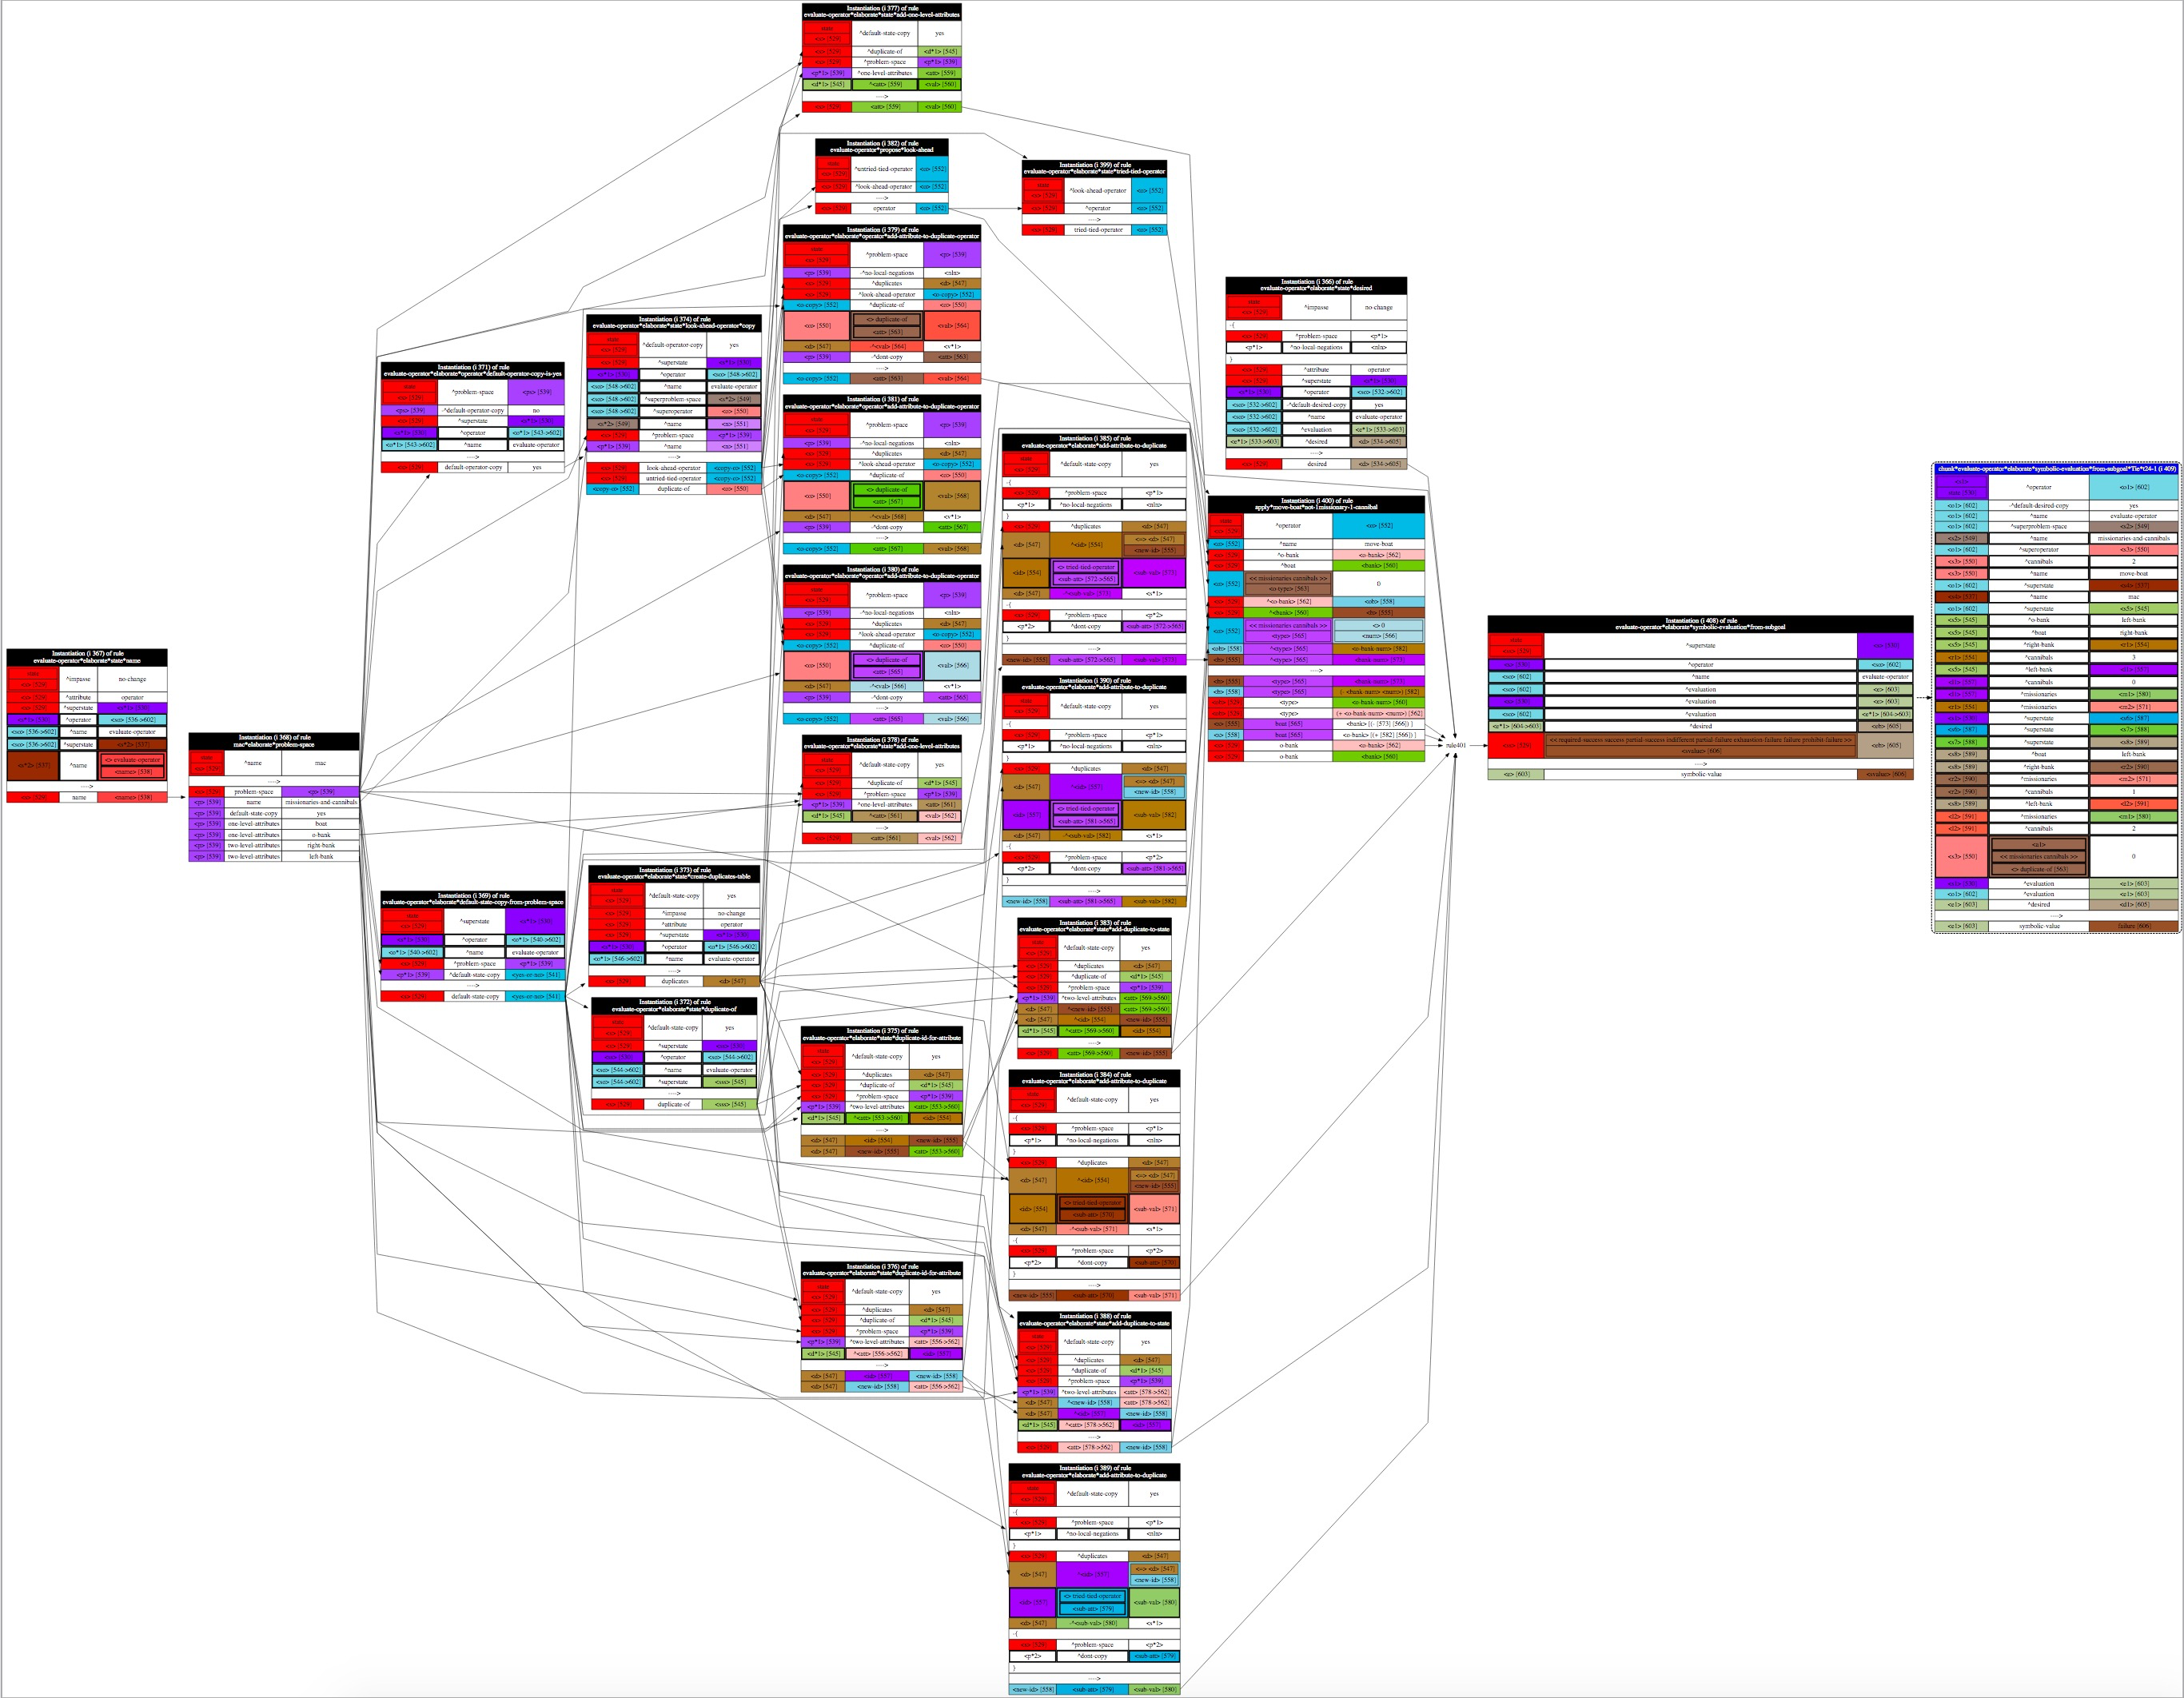
\includegraphics[width=\textwidth]{chunking-trace-identity.png}
	%	}
	\insertcaption{A colored visualization of an explanation trace}
	\label{fig:chunking-viz-identity}
\end{figure}

The \soar{visualize} command can generate two graphical representations of the analysis that chunking performed to learn a rule. While the explainer provides more date, these images are the easiest and most effective ways to quickly understand how a chunk was formed, especially for particularly complex chunks.  The visualizer can create two types of chunking-related images:

%\vspace{-12pt}
\begin{enumerate}
	\item An image that shows the entire instantiation graph at once and how it contributed to the learned rule
	
	Use the command \soar{visualize ebc analysis} to create a very informative graph that shows all rules that fired in a substate with arrows that indicate dependencies between actions in one rule and conditions in others. In addition to all of the dependencies between the rules that fired, this visualization also shows which conditions in the instantiations tested knowledge in the superstate and hence became the basis for a condition in the final learned rule.  Finally, the individual elements in the explanation are color-coded to show which variables share the same identity.


	\item Use the \soar{visualize identity graph} to create a graph that shows how identities were used to determine the variablization of a learned rule. This shows all identities found in the chunk and how the identity analysis joined them based on the problem-solving that occurred. This can be useful in determining why two elements were assigned the same variable.
\end{enumerate}

Note that Soar will automatically attempt to launch a viewer to see the image generated. If you have an editor that can open graphviz files, you can have Soar launch that automatically as well. (Such editors allow you to move things around and lay out the components of the image exactly as you want them.) Your operating system chooses which program to launch based on the file type. 

\textbf{For the visualizer to work, you must have Graphviz and DOT installed}, which are free third-party tools, and both must be available on your path.  To date, the visualizer has only been tested on Mac and Linux.  It is possible that certain systems may not allow Soar to launch an external program.